% This is a template for BU-ECE Technical Report.
%
% Depending on report content and author preference, a BU-ECE report may be
% in one of the two following styles:
%
%   - genuine report based on ``report'' style, i.e., with chapters, much like
%     a thesis; can be single- or double-sided,
%
%   - report based on ``article'' style, i.e., with no chapters (only sections,
%     subsections, etc.), much like a journal or conference paper; can be
%     single- or double-sided.

% =====================================================================

%\documentclass[12pt]{report}          %Single-sided report style (chapters)
%\documentclass[12pt,twoside]{report}  %Double-sided report style (chapters)
%\documentclass[12pt]{article}         %Single-sided article style (no chapters)
\documentclass[12pt,utf8,twoside]{article} %Double-sided article style (no chapters)
\usepackage{ctex}
\usepackage{bu_ece_report}
\usepackage{graphicx}
%----------------------------------------------------------------------------------------
%	配置需要使用的插件包
%----------------------------------------------------------------------------------------
\usepackage{ctex}% 设置中文字体包
\usepackage{geometry}% 页面布局包
\usepackage{graphicx} % 插图包
\usepackage{amsmath,amssymb,amsfonts} % 数学字体、符号包
\usepackage{bm}%公示字体加粗包
\usepackage{chngcntr}%计数器重置包
\usepackage{amsthm}%定理工具包
\newtheorem{theorem}{Theorem}
\newtheorem{lemma}{Lemma}
\usepackage{listings}%代码块工具包
\usepackage{color}%颜色宏包
\usepackage{fontspec}%字体宏包
\usepackage{iitem}%多级列表宏包
%----------------------------------------------------------------------------------------
%	配置文档格式	
%----------------------------------------------------------------------------------------
\pagestyle{headings}
%%%%%%%%%%%%%%%%配置中英文字体%%%%%%%%%%
%默认正文宋体、标题黑体、英文times
%%%%%%注意此处名称不可带符号
\setCJKfamilyfont{KT}{KaiTi_GB2312}             %楷体GB_2312字体
\newcommand{\Kaiti}{\CJKfamily{KT}}
\setCJKfamilyfont{FSgb}{FangSong_GB2312}       %仿宋GB_2312
\newcommand{\FangSgb}{\CJKfamily{FSgb}}
\setCJKfamilyfont{HT}{SimHei}       %黑体
\newcommand{\Heit}{\CJKfamily{HT}}
%%%%%%%%%%%%%%设置段落缩进2字符
\setlength\parindent{2em}
%%%%%%%%%%%%%%%%设置页边距%%%%%%%%%%%%%
\geometry{left=1.91cm,right=1.91cm,top=2.54cm,bottom=2.54cm}
%%%%%%%%%%%%%%%设置多级列表环境%%%%%%%%%%%%%%%
\usepackage{enumerate}
\usepackage{enumitem}
%\setlist[enumerate,1]{label=(\arabic*).,font=\textup,
%	leftmargin=2em,labelsep=1mm,topsep=0mm,itemsep=-0.8mm,itemindent=2em}
%\setlist[enumerate,2]{label=(\alph*).,font=\textup, 
%	leftmargin=2em,labelsep=1mm,topsep=-0.8mm,itemsep=-0.8mm,itemindent=2em}
\setenumerate{fullwidth,label=(\arabic*),itemindent=\parindent,listparindent=\parindent,itemsep=0ex,partopsep=0pt,parsep=0ex, topsep=0em,partopsep=0em}

%%%自定义列表环境
%%%%%%%%%%%%%%%%设置带章节号的图表题注和公式好%%%%%%%%
\renewcommand{\thefigure}{\thesection{}-\arabic{figure}}
\renewcommand{\thetable}{\thesection{}-\arabic{table}}
\renewcommand{\theequation}{\thesection{}-\arabic{equation}}
%%%%%%%%%%%%%%%%配置脚注符号%%%%%%%%%%%
\renewcommand{\thefootnote}{\fnsymbol{footnote}}%配置符号样式
\counterwithin*{footnote}{page}%配置每页脚注计数重置
%%%%%%%%%%%%%%%%自定义命令区域%%%%%%%%%%%%%%%%%%%%%%%

%%%%%%%%%%%%%%%%配置代码块格式%%%%%%%%%%%%%%%%%%%%%%%%%%%%%%%%%%%%%%
\lstset{
	frame = single,					%代码块边框
	%frame = trBL,
	framesep = 2em,					%边框与代码距离	
	%framerule = 0.5pt,				%边框粗细
	language = [11]C++,				%设置C++ 11支持	
	alsolanguage = python,			%设置python支持
	breaklines = true,				%自动换行			
	basicstyle = \footnotesize,		%代码字体大小
	numbers = left,					%行号位置
	numberstyle = \footnotesize,	%行号字体大小
	numbersep = 2pt,				%行号与代码距离 
	xleftmargin = 2em,				%左边距,默认同版芯
	xrightmargin = 2em,				%右边距,默认同版芯
	aboveskip = 0pt,				%上边距
	captionpos = b,					%标题位置bottom
	tabsize = 2,					%table对应的space数	
	basicstyle = \fontspec{Times New Roman},
	keywordstyle = \color[rgb]{0,0,1}\bfseries,	%关键字蓝色加粗
	commentstyle = \color[rgb]{0.133,0.445,0.133}, %注释绿色				
}
% In case an adjustment of vertical or horizontal margins is needed
% due to particular LaTeX/dvips or OS installation, you can uncomment
% and edit the following definitions.
% -------------------------------------------------------------------
%\topmargin       0.00 in
%\oddsidemargin   0.50 in
%\evensidemargin  0.00 in

\begin{document}

% Definitions.
% ------------
\buecedefinitions%
        {VINS-Mono论文及代码解析}
        {Pipeline and code analysis of VINS-Mono}
        {李云天}
        {\today}
        {2019-08} % Number of the report (four year digits and number)

% Box with title to fit the opening in the cover
% (adds an empty page in double-sided printing mode).
% ---------------------------------------------------
\buecereporttitleboxpage

% Title page
% (adds an empty page in double-sided printing mode).
% ---------------------------------------------------
\buecereporttitlepage

% Special page, e.g., if the report is restricted or
% to whom it is dedicated, etc., otherwise skip.
% (adds an empty page in double-sided printing mode).
% ---------------------------------------------------
%\bueceprefacepage{Here comes a special preface page. For example, if the report
%is restricted, then a suitable note can be included. This page can also be used
%to indicate to whom the document is dedicated, etc.}
%
%% Report summary; max. 1 page.
%% (adds an empty page in double-sided printing mode).
%% ---------------------------------------------------
\pagenumbering{roman}
\setcounter{page}{1}
%\buecereportsummary{Summary of the report. Maximum 1 page.}
%
%% Table of contents, list of figures and list of tables.
%% ``\bueceemptypage'' adds empty page in double-sided
%% printing mode and performs ``\clearpage'' in single-sided
%% mode.
%% ------------------------------------------------------
\tableofcontents\bueceemptypage
\listoffigures\bueceemptypage
\listoftables\bueceemptypage

% Switch on running headers for the report:
%   odd pages  - title (lowercase); if too long, use
%                the first few words followed by ``...'',
%   even pages - last names of the authors.
% -------------------------------------------------------
\buecereportheaders

% Introduction.
% -------------
\pagenumbering{arabic}
\setcounter{page}{1}
% pipeline of VINS-Mono
\section{概述}  % Article style
%\chapter{Introduction}  % Report style
\subsection{系统概览}
单目相机和低成本IMU构成了能对空间六自由度状态进行估计的最小传感器单元——惯性视觉导航系统(Visual Inertial Navigation System,VINS)。但距离和位姿直接量测信息的缺乏,给VINS带来了IMU处理、估计器初始化、相机标定和非线性优化等方面的挑战。本文提出了一种鲁棒多功能单目视觉惯性导航系统——VINS-Mono。本方法基于鲁棒初始化和故障恢复,融合紧耦合非线性优化方法、IMU预积分方法以及特征检测方法以获取高精度的视觉惯性里程计。回环检测模块的加入则进一步实现了紧耦合下最小计算量的重定位。此外,本方法还是用四方向位姿图优化加强全局一致性。算法的性能在公开数据集和实际飞行试验中得到了有效验证,并和现有算法进行了对比。
% Following sections, subsections, etc.
% -------------------------------------
单目相机的小尺寸、低成本、易配置等特点使其成为了SLAM领域的最常用传感器,但纯单目视觉系统无法恢复几何尺度;而IMU可以提供几何尺度、角速度等全面的量测信息,同时缓解由于光照变化、特征缺失、运动模糊等带来的视觉跟踪丢失问题。由于单目VINS需要加速度激励才能使几何尺度可观,单目VINS必须在未知的运动而非静止状态下完成初始化,这就给VINS中状态估计器的初始化带来了挑战。

VINS-Mono正是为解决这一问题而诞生,本方法起始于状态估计器的\textbf{在线初始化},核心是基于\textbf{非线性滑窗优化}的\textbf{紧耦合}VIO。该VIO模块不仅提供精确的局部位姿、速度和航向估计,还提供相机-IMU内参和零偏的\textbf{在线修正}。回环检测则基于\textbf{Dow2}词袋实现。重定位基于单目VIO的\textbf{特征级融合}实现以实现最小计算复核下的精确鲁棒回环检测。同时VINS-Mono还加入了\textbf{几何回环}验证模块基于IMU的角度量测优化\textbf{4自由度位姿图}以保证全局一致性。

图\ref{fig.1}给出了VINS的总体结构,系统起始于量测处理模块,包括图像特征的提取和跟踪,以及两图像之间IMU的预积分。随后初始化模块提供位姿、速度、重力矢量、陀螺偏差、3D特征位置等必要的信息供后续基于非线性优化的VIO使用。带有重定位功能的紧耦合VIO模块负责融合预积分的IMU量测、图像特征量测以及回环中重新检测到的图像特征信息。最终,位子图优化基于几何验证重定位结果执行全局优化以消除飘逸。VIO、重定位和位姿图优化分别运行在独立的线程中以保证系统运行的可靠性和实时性。
\subsection{符号约定}
这里首先给出本文中的符号约定。$a$等小写常规字母表示标量,$\bm{x}$等小写加粗字母表示矢量,$\bm{J}$等大写加粗字母表示矩阵。字母上标表示该标量所在的坐标系,$\left(\cdot\right)^w$为世界坐标系,采用N-E-D定义,$z$轴指向重力矢量方向;$\left(\cdot\right)^b$为本体坐标系,采用前右下定义,IMU测量坐标系于本体系一致;$\left(\cdot\right)^w$为相机坐标系,同样采用前右下定义,不同之处在于此处以相机光轴为前。坐标旋转分别采用旋转矩阵$\bm{R}$和四元数$\bm{q}$表示,旋转方向为下标到上标,即$\bm{q}_b^w$表示本体系到世界系的坐标旋转四元数。$\bm{t}_b^w$表示本体系到世界系的坐标平移变换矢量。下标$k$表示当前对应的图像帧,例如$c_k$、$b_k$分别表示第$k$帧图像采集时的本体坐标系和相机坐标系。$\bm{g}=\left[0,0,g\right]^T$为重力矢量。$\otimes$为四元数乘法运算符。使用上标$\hat{\left(\cdot\right)}$表示变量的估计值或测量值,以和实际值区分。

\begin{figure}[htbp]
	\centering
	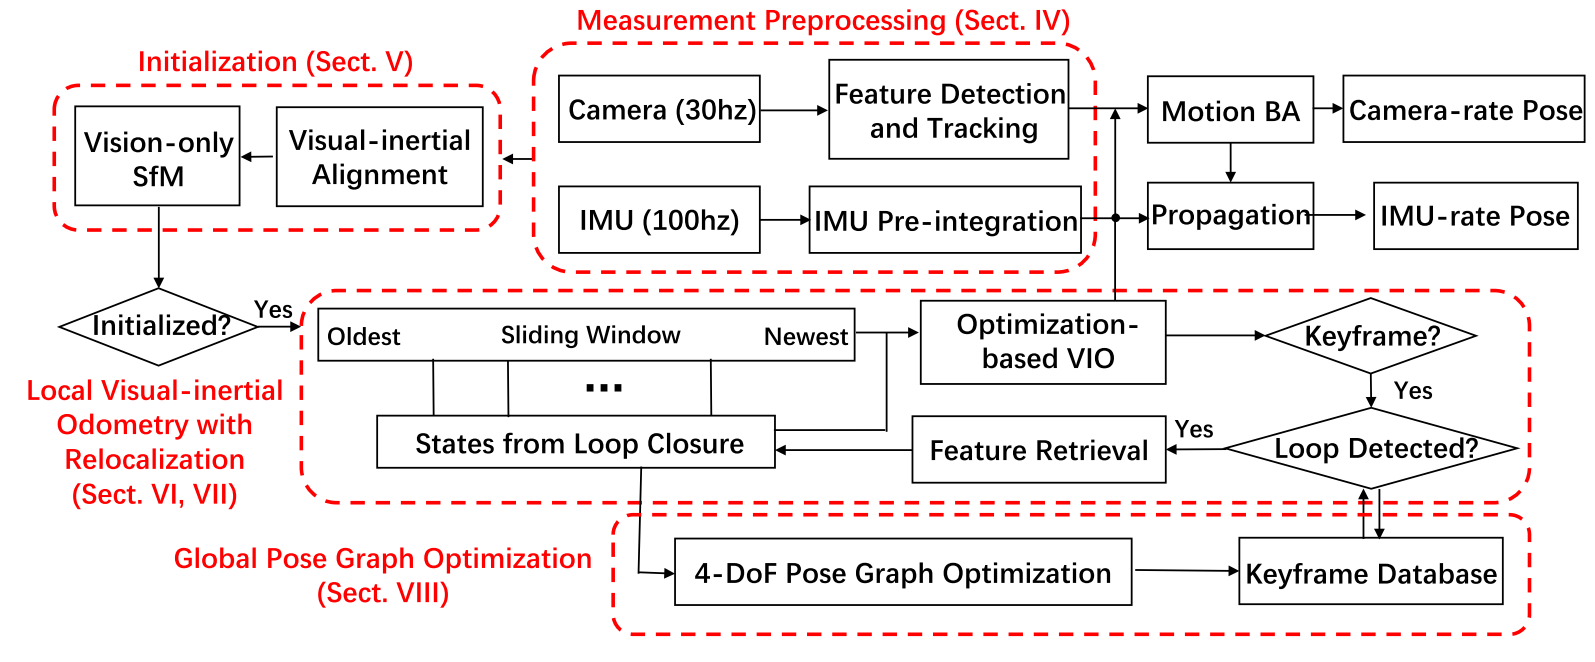
\includegraphics[scale=0.3]{VINS_structure.png}
	\caption{VINS-Mono系统框架}
	\label{fig.1}
\end{figure}      

\section{量测处理}
本节主要介绍连续两帧间IMU和相机的量测处理过程。相机量测处理分为跟踪参考帧关键点(Keypoints)在当前帧中的位置和探测当前帧中新的关键点两部分;IMU量测的处理则主要是在集中在预积分过程。由于低成本IMU中零偏和噪声量级较为接近,这里假设噪声为高斯白噪声,在预积分过程中只考虑器件零偏的影响。
\subsection{视觉前端处理}
对于每一帧新图像,基于KLT稀疏光流法跟踪现有特征;同时采用Shi-Tomasi角点检测检测当前帧中新出现的特征以保证图像中的最小特征数(100-300)。同时,通过设置相邻特征之间的最小像素距离保证特征在图像中均匀分布。2D特征首先经过去畸变处理,随后基于RANSAC算法去除野值量测,最后投影到单位球上。

关键帧的选取则基于以下两个原则。首先,判断两帧之间的平均视差,如果所跟踪的特征在当前帧和上一个参考帧之间的视差超过一定阈值,则将当前帧作为新的关键帧;同时为了分离纯旋转引起的视差变化,对两帧之间的陀螺量测进行积分,补偿旋转的影响。这一旋转补偿只作用于关键帧选取而给位姿估计,因此不会影响位姿估计质量。其次,判断所跟踪的特征数目,若小于一定数量,则将当前帧作为新的关键帧,以防跟踪丢失。
\subsection{IMU预积分}
IMU预积分基于连续时间四元数微分方法实现,相关公式的详细推导参见附录\ref{append.b},这里直接给出结论。
\subsubsection{IMU器件模型}
IMU的量测模型可表示为:
\begin{equation}
\left\{
\begin{aligned}
&\hat{\bm{a}}^b=\bm{a}^b+\bm{b}_a+\bm{R}_w^b\bm{g}^w+\bm{n}_a\\
&\hat{\bm{\omega}}^b=\bm{\omega}^b+\bm{b}_\omega+\bm{n}_\omega
\end{aligned}
\right.
\end{equation}
式中,$\hat{\bm{a}}^b$和$\hat{\bm{\omega}}^b$分别表示IMU的加速度和角速度测量信息;$\bm{a}^b$和$\bm{\omega}^b$分别为载体真实的加速度和角速度;$\bm{b}_a$和$\bm{b}_\omega$分别为加速度计和陀螺仪零偏,建模为随机游走过程:
\begin{equation}
\centering
\left\{
\begin{aligned}
&\bm{n}_{\bm{b}_a}\sim\mathcal{N}\left(\bm{0},\bm{\sigma}_{b_a}^2\right),\bm{n}_{\bm{b}_\omega}\sim\mathcal{N}\left(\bm{0},\bm{\sigma}_{b_\omega}^2\right)\\
&\dot{\bm{b}_a}=\bm{n}_{\bm{b}_a},dot{\bm{b}_\omega}=\bm{n}_{\bm{b}_\omega}
\end{aligned}
\right.
\end{equation}
$\bm{R}_w^b$为世界坐标系到本体坐标系的坐标旋转矩阵;$\bm{g}^w$为世界坐标系下的重力加速度矢量;$\bm{n}_a\sim\mathcal{N}\left(\bm{0},\bm{\sigma}_a^2\right)$和$\bm{n}_\omega\sim\left(\bm{0},\bm{\sigma}_\omega^2\right)$为器件的高斯白噪声。
\subsubsection{IMU预积分项}
由于IMU直接预积分项包含$k$时刻的位姿信息,不便于后端优化,因此使用增量形式的预积分项表达式:
\begin{equation}
\centering
\left\{
\begin{aligned}
&\hat{\bm{\alpha}}_{k+1}^{b_k}=\iint_{t_i\in\left[t_k,t_{k+1}\right]}\left(\bm{R}_{b_{t_i}}^w\left(\hat{\bm{a}}_{t_i}-\bm{b}_a-\bm{n}_a\right)\right)dt^2\\
&\hat{\bm{\beta}}_{k+1}^{b_k}=\int_{t_i\in\left[t_k,t_{k+1}\right]}\left(\bm{R}_{b_{t_i}}^w\left(\hat{\bm{a}}_{t_i}-\bm{b}_a-\bm{n}_a\right)\right)dt\\
&\hat{\bm{\gamma}}_{k+1}^{b_k}=\int_{t_i\in\left[t_k,t_{k+1}\right]}\frac{1}{2}\bm{\Omega}\left(\hat{\bm{\omega}}_{wb}^w-\bm{b}_\omega-\bm{n}_\omega\right)\bm{\gamma}_k^{t_i}dt
\end{aligned}
\right.
\end{equation}
式中$\bm{\alpha}$、$\bm{\beta}$和$\bm{\gamma}$分别为位置、速度和四元数的增量预积分项。
\subsubsection{增量预积分关于零偏的更新}
虽然增量形式的预积分避免了每次后端优化引起$k$时刻位姿变化时都需要重新预积分的问题,但仍需要根据零偏优化数的变化进行更新。为减少计算量,VINS-Mono采取入夏更新策略:当后端优化的IMU零偏变化时,若变化较小,则使用IMU预积分项关于零偏的一阶近似更新预积分项;否则,则按照式\ref{eq.append.b.21}重新积分IMU得到预积分项。IMU预积分关于零偏的线性化更新表达式可以表示为:
\begin{equation}
\left\{
\begin{aligned}
&\hat{\bm{\alpha}}_k^{k+1}\approx\hat{\bm{\alpha}}_k^{k+1}+\bm{J}^{\bm{\alpha}}_{\bm{b}_a}\delta\bm{b}_a+\bm{J}^{\bm{\alpha}}_{\bm{b}_\omega}\delta\bm{b}_\omega\\
&\hat{\bm{\beta}}_k^{k+1}\approx\hat{\bm{\beta}}_k^{k+1}+\bm{J}^{\bm{\beta}}_{\bm{b}_a}\delta\bm{b}_a+\bm{J}^{\bm{\beta}}_{\bm{b}_\omega}\delta\bm{b}_\omega\\
&\hat{\bm{\gamma}}_k^{k+1}=\hat{\bm{\gamma}}_k^{k+1}\otimes\bm{J}^{\bm{\gamma}}_{\bm{b}_\omega}\delta\bm{b}_\omega
\end{aligned}
\right.
\label{eq.2.4}
\end{equation}
\section{估计器初始化}
单目紧耦合VIO是一个高度依赖于精确初始值的非线性系统,VINS-Mono通过IMU预积分和视觉SfM(Structure from Motion)获得的松耦合对准获得。
\subsection{相机与IMU外参对准}
与精确标定的数据集不同,在一些实际应用中,相机和IMU之间外参矩阵的标定精度不够。对于这种情况,VINS-Mono将标定后的外参作为初值,在初始化过程中对其进行进一步优化。由于平移的影响并没有旋转显著,VINS-Mono只考虑IMU与相机之间相对旋转矩阵的标定。

假设相机得到的两帧之间旋转矩阵为$\bm{R}_{c_k}^{c_{k+1}}$,IMU预积分得到的旋转矩阵为$\bm{R}_{b_k}^{b_{k+1}}$,相机和IMU之间的旋转矩阵为$\bm{R}_b^c$,则对于任意两帧图像,均有:
\begin{equation}
\bm{R}_{b_{k+1}}^{b_k}\bm{R^b_c}=\bm{R}_c^b\bm{R}_{c_{k+1}}^{c_k}
\end{equation}
\subsection{滑窗内的纯视觉SfM}
\subsubsection{算法概览}
为了限制算法的计算规模,前端在滑动窗口内仅维持有限数目的图像帧。首先,检测最后一帧图像和窗口内所有其他图像中的特征跟踪情况:若最后一帧图像和任意一个图像帧的稳定跟踪特征超过30个(\textit{程序中设定是15对,这里概念不是很清楚}),且有效视差超过20对,则基于五点法恢复两帧之间的位姿。随后基于五点法恢复的位姿,对这两帧中跟踪到的特征点进行三角化,再基于三角化后的特征点利用PnP算法估计所有帧位姿,最终基于全局BA算法最小化所有特征点的总重投影误差。(这里原文说明的流程并不清楚,究竟是哪些帧之间的位姿,哪一帧向哪一帧的重投影误差,需要进一步参考程序。)由于纯视觉系统缺乏有关世界坐标系的先验信息,这里假设第一帧的相机坐标系(此处是否指的是窗口内的第一帧?)为参考坐标系,所有的相机位姿$\left(\overline{\bm{p}}_{c_k}^{c_0},\bm{q}_{c_k}^{c_0}\right)$和特征点位置均表示在第一帧坐标系下。记相机和IMU之间的外参为$\left(\bm{p}_c^b,\bm{q}_c^b\right)$,则IMU坐标系在$c_0$下的位姿为:
\begin{equation}\begin{aligned}
&\bm{q}_{b_k}^{c_0}=\bm{q}_b^c\otimes\bm{q}_{c_k}^{c_0}\\
&s\overline{\bm{p}}_{b_k}^{c_0}=s\overline{p}_{c_k}^{c_0}-\bm{p}^c_b
\end{aligned}
\end{equation}
\subsubsection{程序解析}
滑窗内的纯视觉SfM包含在GlobalSFM类中,对应头文件和源文件为vins\_estimator/initial文件夹下的initial\_sfm.cpp和initial\_sfm.h,该类只有唯一的一个公共借口函数constructor(),对应的算法流程如下:
\begin{enumerate}
	\item 选取包含$k$个图像帧的滑动窗口,将窗口内的第1帧图像对应的位姿设为基准位姿,记该图像的序号为$l$;利用对极几何约束(五点法或八点法)恢复第$k$帧的相对位姿;
	\item 基于第1帧和第$k$帧的位姿三角化部分特征点的空间位置信息;
	\item 从已三角化的特征点集合中选取能被第2帧图像看到的特征点,基于PnP求解第2帧的相对位姿;
	\item 基于第一帧和第$k$帧的位姿三角化部分特征点的空间位置信息,第2步中已经三角化的特征点会被直接跳过;
	\item 重复上述步骤直到第$k-1$帧,此时滑窗内所有图像帧相对于第1帧的相对位姿均已获得。
	\item 依次基于第1帧位姿和第$i$帧位姿三角化前序过程中剩余的特征点;
	\item 基于现有的特征点空间信息,利用PnP求解窗口内第$l-1$帧图像的相对位姿;
	\item 基于第$l$帧和第$l-1$帧位姿三角化部分特征点的空间信息;
	\item 重复7、8两步直到系统起始时刻的第0帧图像;
	\item 至此,所有图像帧的相对位姿均解算完毕,对于此时仍未三角化的特征点,选择其第一次和最后一次被观测到的图像帧,进行三角化。
	\item 使用Ceres对现有所有图像帧的位姿和空间点的三维坐标进行BA优化。
	
\end{enumerate}
\subsection{惯性视觉对准}
惯性视觉对准的基本思想是将IMU的与积分值与视觉SfM获得了待尺度的数值进行匹配。
\subsubsection{陀螺零偏标定}
考虑窗口内的连续两帧$\bm{b}_k$和$\bm{b}_{k+1}$,我们已经通过纯视觉SfM计算出了对应的旋转$\bm{q}_{b_k}^{c_0}$和$\bm{q}_{b_{k+1}}^{c_0}$,同时IMU预积分也提供了$k$帧到$k+1$帧的相对姿态约束$\bm{\gamma}^{b_k}_{k+1}$,通过最小化两者之间的误差来实现IMU和视觉量测的对准:
\begin{equation}
\min\limits_{\delta\bm{b}_\omega}\sum\limits_{k\in\mathcal{B}}\|\bm{q}_{b_{k+1}}^{c_0}\otimes{\bm{q}_{b_k}^{c_0}}^{-1}\otimes\bm{\gamma}^{b_k}_{k+1}\|^2
\end{equation}
将式\ref{eq.2.4}中的IMU预积分关于陀螺零偏的线性形式带入,则可通过非线性优化方式得到对陀螺零偏的最优估计,再利用新获得的陀螺零偏更新IMU的预积分项。
\subsubsection{速度矢量、重力矢量及几何尺度初始化}

% appendix 
\appendix
\newpage
\section{KLT稀疏光流跟踪算法}
\label{append.a}
\section{基于四元数微分的IMU预积分模型}
\label{append.b}
\subsection{IMU噪声与零偏模型}
IMU的量测模型可表示为:
\begin{equation}
\left\{
\begin{aligned}
&\hat{\bm{a}}^b=\bm{a}^b+\bm{b}_a+\bm{R}_w^b\bm{g}^w+\bm{n}_a\\
&\hat{\bm{\omega}}^b=\bm{\omega}^b+\bm{b}_\omega+\bm{n}_\omega
\end{aligned}
\right.
\end{equation}
式中,$\hat{\bm{a}}^b$和$\hat{\bm{\omega}}^b$分别表示IMU的加速度和角速度测量信息;$\bm{a}^b$和$\bm{\omega}^b$分别为载体真实的加速度和角速度;$\bm{b}_a$和$\bm{b}_\omega$分别为加速度计和陀螺仪零偏,建模为随机游走过程:
\begin{equation}
\centering
\left\{
\begin{aligned}
&\bm{n}_{\bm{b}_a}\sim\mathcal{N}\left(\bm{0},\bm{\sigma}_{b_a}^2\right),\bm{n}_{\bm{b}_\omega}\sim\mathcal{N}\left(\bm{0},\bm{\sigma}_{b_\omega}^2\right)\\
&\dot{\bm{b}_a}=\bm{n}_{\bm{b}_a},\dot{\bm{b}_\omega}=\bm{n}_{\bm{b}_\omega}
\end{aligned}
\right.
\end{equation}
$\bm{R}_w^b$为世界坐标系到本体坐标系的坐标旋转矩阵;$\bm{g}^w$为世界坐标系下的重力加速度矢量;$\bm{n}_a\sim\mathcal{N}\left(\bm{0},\bm{\sigma}_a^2\right)$和$\bm{n}_\omega\sim\left(\bm{0},\bm{\sigma}_\omega^2\right)$为器件的高斯白噪声。
\subsection{四元数左乘与右乘}
假设一个四元数$\bm{q}_a=\left[\begin{array}{cccc}w_a & x_a & y_a & z_a\end{array}\right]^T=\left[\begin{array}{cc}w_a & \bm{v}_a\end{array}\right]^T$,左乘和右乘的矩阵形式分别为:
\begin{equation}
\begin{aligned}
L\left(\bm{q}_a\right)&=\left[\begin{matrix}
w_a & -x_a & -y_a & -z_a\\
x_a &  w_a & -z_a &  y_a\\
y_a &  z_a &  w_a & -x_a\\
z_a & -y_a &  x_a &  w_a
\end{matrix}\right]=w_a\bm{I}+\left[\begin{matrix}
0 & -\bm{v}_a^T\\
\bm{v}_a & \bm{v}_a^\wedge
\end{matrix}\right]\\
R\left(\bm{q}_a\right)&=\left[\begin{matrix}
w_a & -x_a & -y_a & -z_a\\
x_a &  w_a &  z_a & -y_a\\
y_a & -z_a &  w_a &  x_a\\
z_a &  y_a & -x_a &  w_a
\end{matrix}\right]=w_a\bm{I}+\left[\begin{matrix}
0 & -\bm{v}_a^T\\
\bm{v}_a & -\bm{v}_a^\wedge
\end{matrix}\right]
\end{aligned}
\end{equation}
若四元数的实部位于最后,即$\bm{q}_a=\left[\begin{array}{cccc}x_a & y_a & z_a & w_a\end{array}\right]^T=\left[\begin{array}{cc}\bm{v}_a & w_a\end{array}\right]^T$,则对应的左乘和右乘矩阵为:
\begin{equation}
\begin{aligned}
L\left(\bm{q}_a\right)&=\left[\begin{matrix}
  w_a & -z_a &  y_a & x_a\\
  z_a &  w_a & -x_a & y_a\\
 -y_a &  x_a &  w_a & z_a\\
 -x_a & -y_a & -z_a & w_a
\end{matrix}\right]=w_a\bm{I}+\left[\begin{matrix}
\bm{v}_a^\wedge & \bm{v}_a\\
-\bm{v}_a^T & 0
\end{matrix}\right]\\
R\left(\bm{q}_a\right)&=\left[\begin{matrix}
  w_a &  z_a & -y_a & x_a\\
 -z_a &  w_a &  x_a & y_a\\
  y_a & -x_a &  w_a & z_a\\
 -x_a & -y_a & -z_a & w_a
\end{matrix}\right]=w_a\bm{I}+\left[\begin{matrix}
-\bm{v}_a^\wedge & \bm{v}_a\\
-\bm{v}_a^T & 0
\end{matrix}\right]
\end{aligned}
\end{equation}
\subsection{四元数微分}
假设世界坐标系旋转到本体坐标系的旋转轴为$\bm{n}$,旋转角为$\theta$,则对应的旋转四元数为$\bm{q}=\cos\left(\frac{\theta}{2}\right)+\sin\left(\frac{\theta}{2}\right)\bm{n}$,该单位四元数对时间的导数为:
\begin{equation}
\centering
\frac{d\bm{q}}{dt}=-\frac{1}{2}\sin\left(\frac{\theta}{2}\right)\cdot\frac{d\theta}{dt}+\frac{d\bm{n}}{dt}\cdot\sin\left(\frac{\theta}{2}\right)+\bm{n}\cdot\frac{1}{2}\cos\left(\frac{\theta}{2}\right)\cdot\frac{d\theta}{dt}
\end{equation}
式中$-1=\bm{n}\cdot\bm{n}$,$\frac{d\bm{n}}{dt}=0$,$\frac{d\theta}{dt}=\omega^w_wb$,$\omega^w_wb$为世界坐标系下世界坐标系到本体系的旋转角速度。对上式进一步化简有:
\begin{equation}
\centering
\begin{aligned}
\frac{d\bm{q}}{dt}&=\frac{1}{2}\bm{n}\omega_{wb}^w\left(\cos\left(\frac{\theta}{2}\right)+\bm{n}\sin\left(\frac{\theta}{2}\right)\right)\\
&=\frac{1}{2}\bm{\omega}^w_{wb}\bm{q}
\end{aligned}
\end{equation}
由于陀螺测量得到的角速度为本体系下的角速度$\bm{\omega}_{wb}^b$,和世界坐标系下角速度的关系\footnote{假设四元数$\bm{q}$表示世界坐标系到本体坐标系的旋转,即$f^b=\bm{q}f^w\bm{q}^\ast$。而此处矢量本身并未旋转,只因坐标系旋转引起了坐标的变化,相当于坐标系旋转的逆过程,因此有$\bm{w}^b_{wb}=\bm{q}^\ast\bm{w}^w_{wb}\bm{q}$。}可由四元数表示$\bm{q}\bm{\omega}_{wb}^b\bm{q}^\ast=\bm{\omega}_{wb}^w$,带入上式有:
\begin{equation}
\centering
\frac{d\bm{q}}{dt}=\frac{1}{2}\bm{q}\bm{\omega}_{wb}^b\bm{q}^\ast\bm{q}
\end{equation}
利用单位四元数的性质$\bm{q}\bm{q}^{-1}=\bm{q}\bm{q}^\ast=\bm{I}$得到四元数微分和陀螺测量角速度之间的关系为:
\begin{equation}
\centering
\frac{d\bm{q}}{dt}=\frac{1}{2}\bm{q}\bm{\omega}_{wb}^b
\label{eq.append.b.6}
\end{equation}
上式写成矩阵形式为:
\begin{equation}
\centering
\begin{aligned}
\frac{d\bm{q}}{dt}&=\frac{1}{2}\left[\begin{matrix}
0 & -\omega_x & -\omega_y & -\omega_z \\
\omega_x & 0 & \omega_z & -\omega_y \\
\omega_y & -\omega_z & 0 & \omega_x \\
\omega_z & \omega_y & -\omega_x & 0 
\end{matrix}\right]\bm{q}\\
&=\frac{1}{2}\left[\begin{array}{cc}
0 & -{\bm{\omega}_{wb}^b}^T\\
\bm{\omega}_{wb}^b & -{\bm{\omega}_{wb}^b}^\wedge
\end{array}\right]\\
&=\frac{1}{2}\bm{\Omega}\left(\bm{\omega}_{wb}^b\right)\bm{q}
\end{aligned}
\end{equation}
该矩阵形式默认四元数的排列为实部在前。

此外,这里说明下四元数和坐标旋转矩阵之间的关系,假设$w$系旋转到$b$系对应的旋转四元数为$\bm{q}_w^b$,坐标旋转矩阵为$\bm{R}_w^b$,则对于任意一个矢量$\bm{a}$有$\bm{R}_w^b\bm{a}={\bm{q}_w^b}^\ast\bm{a}\bm{q}_w^b$,展开得:
\begin{equation}
\centering
\begin{aligned}
\bm{R}_w^b\bm{a}&=\left[\begin{array}{c}
\left(q_w^2+q_x^2-q_y^2-q_z^2\right)x + 2\left(q_wq_z+q_xq_y\right)y+2\left(q_xq_z-q_2q_y\right)z\\
2\left(q_xq_y-q_wq_z\right)x+\left(q_w^2-q_x^2+q_y^2-q_z^2\right)y+2\left(q_wq_x+q_yq_z\right)z\\
2\left(q_wq_y-q_xq_z\right)x+2\left(q_yq_z-q_wq_x\right)y+\left(q_w^2-q_x^2-q_y^2+q_z^2\right)z
\end{array}\right]\\
&=\left[\begin{array}{ccc}
\left(q_w^2+q_x^2-q_y^2-q_z^2\right) & 2\left(q_wq_z+q_xq_y\right) & 2\left(q_xq_z-q_2q_y\right)\\
2\left(q_xq_y-q_wq_z\right) & \left(q_w^2-q_x^2+q_y^2-q_z^2\right) & 2\left(q_wq_x+q_yq_z\right)\\
2\left(q_wq_y-q_xq_z\right) & 2\left(q_yq_z-q_wq_x\right) & \left(q_w^2-q_x^2-q_y^2+q_z^2\right)
\end{array}\right]\left[\begin{array}{c}x\\y\\z\end{array}\right]
\end{aligned}
\end{equation}
\subsection{四元数微分的毕卡算法}
式\ref{eq.append.b.6}所表示的四元数微分方程可采用毕卡级数求解,这里省略详细的推导过程,直接给出四元数的毕卡积分解:
\begin{equation}
\bm{q}_{t_{k+1}}=e^{\frac{1}{2}\int_{t_k}^{t_{k+1}}\bm{\Omega}\left(\bm{\omega_{wb}^b}\right)dt}\bm{q}_{t_k}
\label{eq.append.b.10}
\end{equation}
记$\Delta\bm{\Theta}=\int_{t_k}^{t_{k+1}}\bm{\Omega}\left(\bm{\omega_{wb}^b}\right)dt$,则:
\begin{equation}
\centering
\begin{aligned}
\Delta\Theta&=\int_{k}^{k+1}\left[\begin{matrix}
0 & -\omega_x & -\omega_y & -\omega_z \\
\omega_x & 0 & \omega_z & -\omega_y \\
\omega_y & -\omega_z & 0 & \omega_x \\
\omega_z & \omega_y & -\omega_x & 0 
\end{matrix}\right]dt\\
&\approx\left[\begin{matrix}
0 & -\Delta\theta_x & -\Delta\theta_y & -\Delta\theta_z\\
\Delta\theta_x & 0 & \Delta\theta_z & -\Delta\theta_y\\
\Delta\theta_y & -\Delta\theta_z & 0 & \Delta\theta_x\\
\Delta\theta_z & \Delta\theta_y & -\Delta\theta_x & 0
\end{matrix}\right]
\end{aligned}
\end{equation}
$\Delta\bm{\theta}=\left[\begin{array}{ccc}\Delta\theta_x & \Delta\theta_y&\Delta\theta_z\end{array}\right]$称为采样时间$\left[t_k, t_{k+1}\right]$内的角增量。将上式带入式\ref{eq.append.b.10}中并对其进行泰勒展开有:
\begin{equation}
\centering
\begin{aligned}
\bm{q}_{t_{k+1}}&=e^{\frac{1}{2}\Delta\bm{\Theta}}\bm{q}_{t_k}\\
&=\left(\bm{I}+\frac{\frac{1}{2}\Delta\bm{\Theta}}{1!}+\frac{\left(\frac{1}{2}\Delta\bm{\Theta}\right)^2}{2!}+\frac{\left(\frac{1}{2}\Delta\bm{\Theta}\right)^3}{3!}+\frac{\left(\frac{1}{2}\Delta\bm{\Theta}\right)^4}{4!}+o\left(\frac{1}{2}\Delta\bm{\Theta}\right)\right)\bm{q}_{t_k}\\
\end{aligned}
\label{eq.append.b.12}
\end{equation}
上式中,$o\left(\frac{1}{2}\Delta\bm{\Theta}\right)$为高阶小量。$\Delta\bm{\Theta}$的幂函数存在一定的规律:
\begin{equation}
\centering
\begin{aligned}
\Delta\bm{\Theta}^2&=-\Delta\Theta^2\bm{I}\\
\Delta\bm{\Theta}^3&=-\Delta\Theta^2\Delta\bm{\Theta}\\
\Delta\bm{\Theta}^4&=-\Delta\Theta^4\bm{I}\\
\Delta\bm{\Theta}^5&=\Delta\Theta^4\Delta\bm{\Theta}\\
\cdots
\end{aligned}
\end{equation}
将上式带入式\ref{eq.append.b.12}并合并包含和不包含$\Delta\bm{\Theta}$的同类项有:
\begin{equation}
\centering
\begin{aligned}
\bm{q}_{t_{k+1}}&=\left\{\bm{I}\left(1-\frac{\left(\frac{\Delta\theta}{2}\right)^2}{2!}+\frac{\left(\frac{\Delta\theta}{2}\right)^4}{4!}-\frac{\left(\frac{\Delta\theta}{2}\right)^6}{6!}+\cdots\right)+\frac{\Delta\bm{\Theta}}{2}\left(\frac{\left(\frac{\Delta\theta}{2}\right)}{1!}-\frac{\left(\frac{\Delta\theta}{2}\right)^3}{3!}+\frac{\left(\frac{\Delta\theta}{2}\right)^5}{5!}-\cdots\right)\frac{2}{\Delta\theta}\right\}\bm{q}_{t_k}\\
&=\left(\bm{I}\cos\frac{\Delta\theta}{2}+\Delta\bm{\Theta}\frac{\sin\frac{\Delta\theta}{2}}{\Delta\theta}\right)\bm{q}_{t_k}
\end{aligned}
\end{equation}
上式即为完整形式的四元数角增量毕卡算法。但实际应用中,为了避免计算三角函数,通常直接取近似解:
\begin{enumerate}
	\item 一阶近似毕卡算法:
	\begin{equation}
		\bm{q}_{t_k+1}=\left(\bm{I}+\frac{\Delta\bm{\Theta}}{2}\right)\bm{q}_{t_k}
	\end{equation}
	\item 二阶近似毕卡算法:
	\begin{equation}
	\bm{q}_{t_k+1}=\left[\bm{I}\left(1-\frac{\Delta\theta^2}{8}\right)+\frac{\Delta\bm{\Theta}}{2}\right]\bm{q}_{t_k}
	\end{equation}	
	\item 三阶近似毕卡算法:
	\begin{equation}
	\bm{q}_{t_k+1}=\left[\bm{I}\left(1-\frac{\Delta\theta^2}{8}\right)+\left(\frac{1}{2}-\frac{\Delta\theta^2}{48}\right)\Delta\bm{\Theta}\right]\bm{q}_{t_k}
	\end{equation}
	\item 四阶近似毕卡算法:
	\begin{equation}
	\bm{q}_{t_k+1}=\left[\bm{I}\left(1-\frac{\Delta\theta^2}{8}+\frac{\Delta\theta^4}{384}\right)+\left(\frac{1}{2}-\frac{\Delta\theta^2}{48}\right)\Delta\bm{\Theta}\right]\bm{q}_{t_k}
	\end{equation}
\end{enumerate}
其中,将一阶毕卡算法写成四元数乘法形式为:
\begin{equation}
	\bm{q}_{t_{k+1}}=\bm{q}_{t_k}\otimes\left[\begin{array}{c}
	1\\
	\frac{\Delta\theta_x}{2}\\
	\frac{\Delta\theta_y}{2}\\
	\frac{\Delta\theta_z}{2}
	\end{array}\right]\\
\end{equation}
进一步离散化有:
\begin{equation}
	\bm{q}_{t_{k+1}}=\bm{q}_{t_k}\otimes\left[\begin{array}{c}
	1\\
	\frac{1}{2}\bm{\omega}_{wb}^b\delta t
	\end{array}\right]
\end{equation}
\subsection{基于四元数的IMU预积分}
\subsubsection{连续时间形式}
载体的位置、速度和姿态四元数在时间区间$\left[t_k,t_{k+1}\right]$内的传播方程为:
\begin{equation}
\centering
\left\{
\begin{aligned}
&\bm{p}_{k+1}^w=\bm{p}_k^w+\bm{v}_k^w\Delta t_k+\iint_{t_i\in\left[t_k,t_{k+1}\right]}\left(\bm{R}_{b_{t_i}}^w\left(\hat{\bm{a}}_{t_i}-\bm{b}_a-\bm{n}_a\right)-\bm{g}^w\right)dt^2\\
&\bm{v}_{k+1}^w=\bm{v}_k^w+\int_{t_i\in\left[t_k,t_{k+1}\right]}\left(\bm{R}_{b_{t_i}}^w\left(\hat{\bm{a}}_{t_i}-\bm{b}_a-\bm{n}_a\right)-\bm{g}^w\right)dt\\
&\bm{q}_w^{b_{k+1}}=\bm{q}_w^{b_{k}}\otimes\int_{t_i\in\left[t_k,t_{k+1}\right]}\frac{1}{2}\bm{\Omega}\left(\hat{\bm{\omega}}_{wb}^w-\bm{b}_\omega-\bm{n}_\omega\right)\bm{q}_k^wdt
\end{aligned}
\right.
\label{eq.append.b.11}
\end{equation}
式中${\bm{q}_w^{b_{k+1}}}$为世界坐标系到本体坐标系的旋转四元数,$\otimes$表示四元数乘法,$\bm{\Omega}\left(\bm{\omega}\right)$为上一小节中由$\bm{\omega}$组成的齐次矩阵,$\bm{b}_k$和$\bm{b}_{k+1}$分别为第$k$帧和第$k+1$帧对应的体坐标系,$\bm{b}_{t_i}$为$t_i$时刻的体坐标系。

可以看出,IMU的由第$k$帧向第$k+1$帧的状态传播需要第$k$帧的旋转、位置和速度信息,这使得后端优化时,每当$k$帧位姿优化完后均需要重新计算$k+1$的相关变量;而若将\ref{eq.append.b.11}中右侧的积分项表示在$k$帧对应的本体系下,则该项不包含任何需要后端优化的位姿变量而只依赖于IMU的量测信息,更加便于后端优化处理。因此,增量形式的IMU状态传播方程为:
\begin{equation}
\centering
\left\{
\begin{aligned}
	&\bm{R}_w^{b_k}\bm{p}_{k+1}^w=\bm{R}_w^{b_k}\left(\bm{p}_k^w+\bm{v}_k^w\Delta t_k-\frac{1}{2}\bm{g}^w\Delta t_k^2\right)+\hat{\bm{\alpha}}_{k+1}^{b_k}\\
	&\bm{R}_w^{b_k}\bm{v}_{k+1}^w=\bm{R}_w^{b_k}\left(\bm{v}_k^w-\bm{g}^w\Delta t_k\right)+\hat{\bm{\beta}}_{k+1}^{b_k}\\
	&\bm{q}_{b_{k}}^w\otimes\bm{q}_w^{b_{k+1}}=\hat{\bm{\gamma}}_{k+1}^{b_k}
\end{aligned}
\right.
\end{equation}
式中,$\bm{\alpha}_{k+1}^{b_k}$、$\bm{\beta}_{k+1}^{b_k}$和$\bm{\gamma_{k+1}^{b_k}}$分别为$b_k$坐标系下第$k$和$k+1$帧之间IMU的预积分项:
\begin{equation}
\centering
\left\{
\begin{aligned}
&\hat{\bm{\alpha}}_{k+1}^{b_k}=\iint_{t_i\in\left[t_k,t_{k+1}\right]}\left(\bm{R}_{b_{t_i}}^w\left(\hat{\bm{a}}_{t_i}-\bm{b}_a-\bm{n}_a\right)\right)dt^2\\
&\hat{\bm{\beta}}_{k+1}^{b_k}=\int_{t_i\in\left[t_k,t_{k+1}\right]}\left(\bm{R}_{b_{t_i}}^w\left(\hat{\bm{a}}_{t_i}-\bm{b}_a-\bm{n}_a\right)\right)dt\\
&\hat{\bm{\gamma}}_{k+1}^{b_k}=\int_{t_i\in\left[t_k,t_{k+1}\right]}\frac{1}{2}\bm{\Omega}\left(\hat{\bm{\omega}}_{wb}^w-\bm{b}_\omega-\bm{n}_\omega\right)\bm{\gamma}_k^{t_i}dt
\end{aligned}
\right.
\label{eq.append.b.21}
\end{equation}
可以看出,\ref{eq.append.b.21}中的IMU预积分项只和实际IMU期间量测以及IMU零偏有关。当后端优化的IMU零偏变化时,若变化较小,则使用IMU预积分项关于零偏的一阶近似更新预积分项;否则,则按照式\ref{eq.append.b.21}重新积分IMU得到预积分项。IMU预积分关于零偏的线性化更新表达式可以表示为:
\begin{equation}
\left\{
\begin{aligned}
&\hat{\bm{\alpha}}_k^{k+1}\approx\hat{\bm{\alpha}}_k^{k+1}+\bm{J}^{\bm{\alpha}}_{\bm{b}_a}\delta\bm{b}_a+\bm{J}^{\bm{\alpha}}_{\bm{b}_\omega}\delta\bm{b}_\omega\\
&\hat{\bm{\beta}}_k^{k+1}\approx\hat{\bm{\beta}}_k^{k+1}+\bm{J}^{\bm{\beta}}_{\bm{b}_a}\delta\bm{b}_a+\bm{J}^{\bm{\beta}}_{\bm{b}_\omega}\delta\bm{b}_\omega\\
&\hat{\bm{\gamma}}_k^{k+1}=\hat{\bm{\gamma}}_k^{k+1}\otimes\bm{J}^{\bm{\gamma}}_{\bm{b}_\omega}\delta\bm{b}_\omega
\end{aligned}
\right.
\label{eq.append.b.13}
\end{equation}
\subsubsection{离散时间形式}
为了便于实际程序的执行,需要将上述连续形式的预积分方程改写为离散形式,由于噪声均值为零,预积分中可以忽略不计,因此两个IMU量测时刻$i$和$i+1$之间离散形式的IMU预积分方程为:
\begin{equation}
\centering
\left\{
\begin{aligned}
&\bm{p}_{i+1}^w=\bm{p}_i^w+\bm{v}_i^w\Delta t_i+\frac{1}{2}\overline{\bm{a}}_{t_i}\delta t^2\\
&\bm{v}_{i+1}^w=\bm{v}_i^w+\overline{\bm{a}}_{t_i}\delta t\\
&\bm{q}_w^{b_{i+1}}=\bm{q}_w^{b_{i}}\otimes\left[\begin{array}{c}1\\\frac{1}{2}\overline{\bm{\omega}}_{t_i}\delta t
\end{array}\right]
\end{aligned}
\right.
\end{equation}
式中,$\overline{\bm{a}}_{t_i}$和$\overline{\bm{\omega}}_{t_i}$分别表示离散区间内的离散加速度,具体表达形式由离散方法决定:
\begin{enumerate}
	\item 欧拉法:
	\begin{equation}
	\centering
	\left\{
	\begin{aligned}
	&\overline{\bm{a}}_{t_i}=\bm{R}_{b_{t_i}}^w\left(\hat{\bm{a}}_{t_i}-\bm{b}_a\right)-\bm{g}^w\\
	&\overline{\bm{\omega}}_{t_i}=\hat{\bm{\omega}}_{t_i}-\bm{b}_\omega
	\end{aligned}
	\right.
	\end{equation}
	\item 中值法:
	\begin{equation}
	\centering
	\left\{
	\begin{aligned}
	&\overline{\bm{a}}_{t_i}=\frac{1}{2}\left[\bm{R}_{b_{t_i}}^w\left(\hat{\bm{a}}_{t_i}-\bm{b}_a\right)+\bm{R}_{b_{t_{i+1}}}^w\left(\hat{\bm{a}}_{t_{i+1}}-\bm{b}_a\right)\right]-\bm{g}^w\\
	&\overline{\bm{\omega}}_{t_i}=\frac{1}{2}\left(\hat{\bm{\omega}}_{t_i}+\hat{\bm{\omega}}_{t_{i+1}}\right)-\bm{b}_\omega
	\end{aligned}
	\right.
	\end{equation}
\end{enumerate}
同理,可得到离散的增量形式IMU预积分方程为:
\begin{equation}
\centering
\left\{
\begin{aligned}
&\hat{\bm{\alpha}}_{i+1}^{b_k}=\hat{\bm{\alpha}}_i^{b_k}+\hat{\bm{\beta}}_i^{b_k}\delta t+\frac{1}{2}\overline{\bm{a}}_i\delta t^2\\
&\hat{\bm{\beta}}_{i+1}^{b_k}=\hat{\bm{\beta}}_i^{b_k}+\overline{\bm{a}}_i\delta t\\
&\hat{\bm{\gamma}}_{i+1}^{b_k}=\hat{\bm{\gamma}}_i^{b_k}\otimes\left[\begin{array}{c}1\\\frac{1}{2}\overline{\bm{\omega}}_i\delta t\end{array}\right]
\end{aligned}
\right.
\end{equation}
同样有欧拉法和中值法两种离散形式:
\begin{enumerate}
	\item 欧拉法:
	\begin{equation}
	\centering
	\left\{
	\begin{aligned}
	&\overline{\bm{a}}_i=\bm{R}\left(\hat{\bm{\gamma}}_i^{b_k}\right)\left(\hat{\bm{a}}_i-\bm{b}_a\right)\\
	&\overline{\bm{\omega}}_i=\hat{\bm{\omega}}_i-\bm{b}_\omega
	\end{aligned}
	\right.
	\end{equation}
	\item 中值法:
	\begin{equation}
	\centering
	\left\{
	\begin{aligned}
	&\overline{\bm{a}}_i=\frac{1}{2}\left[\bm{R}\left(\hat{\bm{\gamma}}_i^{b_k}\right)\left(\hat{\bm{a}}_i-\bm{b}_a\right)+\bm{R}\left(\hat{\bm{\gamma}}_{i+1}^{b_k}\right)\left(\hat{\bm{a}}_{i+1}-\bm{b}_a\right)\right]\\
	&\overline{\bm{\omega}}_i=\frac{1}{2}\left(\hat{\bm{\omega}}_i+\hat{\bm{\omega}}_{i+1}\right)-\bm{b}_\omega
	\end{aligned}
	\right.
	\end{equation}
\end{enumerate}
\subsection{IMU预积分误差动力学方程与协方差矩阵}
在VINS的优化中,由于采用马氏距离构建二乘函数,需要对状态的协方差矩阵进行更新,而协方差矩阵的一步预测依赖于状态的误差动力学方程,因此这里我们首先就IMU预积分项的误差动力学方程进行推导。涉及的状态量包括位置增量$\bm{\alpha}_{k+1}^{b_k}$、速度增量$\bm{\beta}_{k+1}^{b_k}$、姿态增量$\bm{\theta}_{k+1}^{b_k}$、加速度计零偏$\bm{b}_a$和陀螺仪零偏$\bm{b_\omega}$,其中由于陀螺器件测量为角增量,这里使用角增量$\bm{\theta}_{k+1}^{b_k}$代替四元数增量$\bm{\gamma}_{k+1}^{b_k}$。
\subsubsection{连续时间形式}
由于我们需要求解的是上述各增量的误差动力学方程,因此系统状态空间矢量可记为\footnote{由于增量表示的是$k+1$和$k$之间的相对值,这里为了书写方便,下标使用$k$而非前面$k+1$,同时改用下标$t$表示IMU测量时刻,以区别图像帧时刻$k$,但两者本质上是同一个量。}。
\begin{equation}
\delta\bm{x}=\left[\begin{array}{ccccccccc}
\delta\bm{\alpha}_t^{b_k} & \delta\bm{\beta}_t^{b_k} & \delta\bm{\theta}_t^{b_k} & \delta\bm{b}_a & \delta\bm{b}_\omega & \bm{n}_a & \bm{n}_\omega & \bm{n}_{\bm{b}_a} & \bm{n}_{\bm{b}_\omega}
\end{array}\right] 
\end{equation}
由于导数运算的顺序可以交换,即$\delta\dot{\bm{a}}=\dot{\delta\bm{a}}$,我们可以先求当前变量的时间导数,再求其对各状态量的偏导数。
\begin{enumerate}
	\item \textbf{位置增量误差}$\delta\bm{\alpha}_t^{b_k}$
	
	位置增量的时间导数为$\dot{\bm{\alpha}}_t^{b_k}=\bm{\beta}_t^{b_k}$,显然,除了偏导数$\delta\dot{\bm{\alpha}}_t^{b_k}/\delta\bm{\beta}_t^{b_k}=\bm{I}$外,位置增量的导数对其余状态增量的导数为零,即其余状态增量的变化对位置增量误差的导数没有贡献.
	\item \textbf{速度增量误差}$\delta\bm{\beta}_t^{b_k}$
	
	速度增量的时间导数为$\dot{\bm{\beta}}_t^{b_k}=\bm{R}_{b_t}^{b_k}\left(\hat{\bm{a}}_t-\bm{b}_a-\bm{n}_a\right)$,可以看出非零偏导数共有三项,分别为:
	\begin{equation}
	\begin{aligned}
	\frac{\delta\bm{\beta}_t^{b_k}}{\delta\bm{\theta}_k^{b_k}}&=-\bm{R}_{b_t}^{b_k}\left(\hat{\bm{a}}_t-\bm{b}_a-\bm{n}_a\right)\\
	&\approx-\bm{R}_{b_t}^{b_k}\left(\hat{\bm{a}}_t-\bm{b}_a\right)\\
	\frac{\delta\bm{\beta}_t^{b_k}}{\bm{b}_a}&=-\bm{R}_{b_t}^{b_k}\\
	\frac{\delta\bm{\beta}_t^{b_k}}{\bm{n}_a}&=-\bm{R}_{b_t}^{b_k}
	\end{aligned}
	\end{equation}
	其中,由于状态递推的本质是随机变量均值的传播,而$\bm{n}_a$是零均值的高斯白噪声,可作为零值处理。
	\item \textbf{角增量误差}$\delta\bm{\theta}_t^{b_k}$
	
	由于角增量的运算中涉及四元数的乘法,使用导数微分定义求解会比较复杂,这里我们换一种思路,假设无任何偏差的四元数时间导数和带各项扰动的四元数时间导数分别为$\dot{\bm{q}}_n$和$\dot{\bm{q}}_t$,则:
	\begin{equation}
	\begin{aligned}
	\dot{\bm{q}}_t&=\frac{1}{2}\underbrace{\bm{q}\otimes\delta\bm{q}}_{\delta\bm{\theta}}\otimes\left[\begin{array}{c}
	0\\\hat{\bm{\omega}}-\bm{b}_\omega-\bm{n}_\omega-\delta\bm{b}_\omega	
	\end{array}\right]\\
	\dot{\bm{q}}_n&=\frac{1}{2}\bm{q}\otimes\left[\begin{array}{c}
	0\\\hat{\bm{\omega}}-\bm{b}_\omega
	\end{array}\right]	
	\end{aligned}
	\end{equation}
	同时,$\dot{\bm{q}}_t$又可表示为:
	\begin{equation}
	\begin{aligned}
	\dot{\bm{q}}_t&=\frac{\partial\left(\bm{q}\otimes\delta\bm{q}\right)}{\partial t}=\dot{\bm{q}}\otimes\delta\bm{q}+\bm{q}\otimes\dot{\delta\bm{q}}\\
	&=\frac{1}{2}\bm{q}\otimes\left[\begin{array}{c}
	0\\\bm{\omega}-\bm{b}_\omega
	\end{array}\right]\otimes\delta\bm{q}+\bm{q}\otimes\dot{\delta\bm{q}}
	\end{aligned}
	\end{equation}
	令上述两式相等可得到:
	\begin{equation}
	\begin{aligned}
	&\frac{1}{2}\bm{q}\otimes\delta\bm{q}\otimes\left[\begin{array}{c}
	0\\\hat{\bm{\omega}}-\bm{b}_\omega-\bm{n}_\omega-\delta\bm{b}_\omega	
	\end{array}\right]=\frac{1}{2}\bm{q}\otimes\left[\begin{array}{c}
	0\\\bm{\omega}-\bm{b}_\omega
	\end{array}\right]\otimes\delta\bm{q}+\bm{q}\otimes\dot{\delta\bm{q}}\\
	\Rightarrow&\frac{1}{2}\delta\bm{q}\otimes\left[\begin{array}{c}
	0\\\hat{\bm{\omega}}-\bm{b}_\omega-\bm{n}_\omega-\delta\bm{b}_\omega	
	\end{array}\right]=\frac{1}{2}\left[\begin{array}{c}
	0\\\bm{\omega}-\bm{b}_\omega
	\end{array}\right]\otimes\delta\bm{q}+\dot{\delta\bm{q}}\\
	\Rightarrow&2\dot{\delta}\bm{q}=\delta\bm{q}\otimes\left[\begin{array}{c}
	0\\\hat{\bm{\omega}}-\bm{b}_\omega-\bm{n}_\omega-\delta\bm{b}_\omega	
	\end{array}\right]-\left[\begin{array}{c}
	0\\\bm{\omega}-\bm{b}_\omega
	\end{array}\right]\otimes\delta\bm{q}\\
	\Rightarrow&2\dot{\delta\bm{q}}=\mathcal{R}\left(\left[\begin{array}{c}
	0\\\hat{\bm{\omega}}-\bm{b}_\omega-\bm{n}_\omega-\delta\bm{b}_\omega	
	\end{array}\right]\right)\delta\bm{q}-\mathcal{L}\left(\left[\begin{array}{c}
	0\\\bm{n}_\omega+\delta\bm{b}_\omega
	\end{array}\right]\right)\delta\bm{q}\\
	\Rightarrow&2\dot{\delta\bm{q}}=\left[\begin{matrix}
		0 & \left(\bm{n}_\omega+\delta\bm{b}_\omega\right)^T\\
		-\left(\bm{n}_\omega-\delta\bm{b}_\omega\right) & -\left(2\hat{\bm{\omega}}-2\bm{b}_\omega-\bm{n}_\omega-\delta\bm{b}_\omega\right)^\wedge\\
		\end{matrix}\right]\left[\begin{array}{c}
		1\\\frac{\delta\bm{\theta}}{2}
		\end{array}\right]\\
	\end{aligned}	
	\end{equation}
	将$\dot{\delta\bm{q}}=\left[\begin{array}{c}
	0\\\frac{1}{2}\dot{\delta\bm{\theta}}
	\end{array}\right]$带入上式可以并忽略零均值项$\bm{n}_\omega$以及二阶小量$\delta\bm{b}_\omega\delta\bm{\theta}$可以得到:
	\begin{equation}
	\begin{aligned}
	\left[\begin{array}{c}
	0\\\dot{\delta\bm{\theta}}\end{array}\right]&=\left[\begin{matrix}
	0 & \left(\bm{n}_\omega+\delta\bm{b}_\omega\right)^T\\
	-\left(\bm{n}_\omega-\delta\bm{b}_\omega\right) & -\left(2\hat{\bm{\omega}}-2\bm{b}_\omega-\bm{n}_\omega-\delta\bm{b}_\omega\right)^\wedge\\
	\end{matrix}\right]\left[\begin{array}{c}
	1\\\frac{\delta\bm{\theta}}{2}
	\end{array}\right]\\
	\Rightarrow\dot{\delta\bm{\theta}}&\approx-\left(\hat{\bm{\omega}}-\bm{b}_\omega\right)^\wedge\delta\bm{\theta}-\bm{n}_\omega-\delta\bm{b}_\omega
	\end{aligned}
	\end{equation}
	\item \textbf{加速度计零偏误差}$\delta\bm{b}_a$:根据IMU的器件模型有$\delta\dot{\bm{b}}_a=\bm{n}_{\bm{b}_a}$。
	\item \textbf{陀螺零偏误差}$\delta\bm{b}_\omega$:同样根据IMU的器件模型有$\delta\dot{\bm{b}}_\omega=\bm{n}_{\bm{b}_\omega}$。
\end{enumerate}

至此,我们已经获得了所有非零均值状态量动力学方程,写成矩阵形式为:
\begin{equation}
\begin{aligned}
\left[\begin{array}{c}
\delta\dot{\bm{\alpha}}_t^{b_k}\\\delta\dot{\bm{\beta}}_t^{b_k}\\\delta\dot{\bm{\theta}}_t^{b_k}\\
\delta\dot{\bm{b}_a}\\\delta\dot{\bm{b}_\omega}
\end{array}\right]&=\left[\begin{matrix}
0 & \bm{I} & 0 & 0 & 0\\
0 & 0 & -\bm{R}_{b_t}^{b_k}\left(\hat{\bm{a}}_t-\bm{b}_a\right)^\wedge & -\bm{R}_{b_t}^{b_k} & 0\\
0 & 0 & -\left(\hat{\bm{\omega}}_t-\bm{b}_\omega\right)^\wedge & 0 & -\bm{I}\\
0 & 0 & 0 & 0 & 0\\
0 & 0 & 0 & 0 & 0
\end{matrix}\right]\left[\begin{array}{c}
\delta\bm{\alpha}_t^{b_k}\\\delta\bm{\beta}_t^{b_k}\\\delta\bm{\theta}_t^{b_k}\\
\delta\bm{b}_a\\\delta\bm{b}_\omega
\end{array}\right]\\
&+\left[\begin{matrix}
0 & 0 & 0 & 0\\
-\bm{R}_{b_t}^{b_k} & 0 & 0 & 0\\
0 & -\bm{I} & 0 & 0\\
0 & 0 & \bm{I} & 0\\
0 & 0 & 0 & \bm{I}
\end{matrix}\right]\left[\begin{array}{c}
\bm{n}_a\\\bm{n}_\omega\\\bm{n}_{\bm{b}_a}\\\bm{n}_{\bm{b}_\omega}
\end{array}\right]\\
\Rightarrow\dot{\delta\bm{x}}_t&=\bm{f}_t\delta\bm{x}_t+\bm{v}_t\bm{n}_t
\end{aligned}\end{equation}
根据导数的定义,可以将上式改写为递推形式:
\begin{equation}
\begin{aligned}
\frac{\delta\bm{x}_{t+1}-\delta\bm{x}_t}{\delta t}&=\bm{f}_t\delta\bm{x}_t+\bm{v}_t\bm{n}_t\\
\delta\bm{x}_{t+1}&=\delta\bm{x}_t+\bm{f}_t\delta\bm{x}_t\delta t + \bm{v}_t\bm{n}_t\delta t\\
&=\underbrace{\left(\bm{I}+\bm{f}_t\delta t\right)}_{\bm{F}_t}\delta\bm{x}_t+\underbrace{\bm{v}_t\delta t}_{\bm{V}_t}\bm{n}_t
\end{aligned}
\end{equation}
可以看出,上式是一个标准的状态空间模型,给出了随机变量均值的传播方程;同样,我们可以直接写出随机变量方差的传播方程:
\begin{equation}
	\begin{aligned}
	\bm{P}_{t+1}&=\bm{F}_t\bm{P}_t\bm{F}_t^T+\bm{V}_t\bm{Q}_t\bm{V}_t^T\\
	\bm{P}_0&=\bm{0}\\
	\bm{Q}_0&=\left[\begin{matrix}
	\sigma_a^2 & 0 & 0 & 0\\
	0 & \sigma_\omega^2 & 0 & 0\\
	0 & 0 & \sigma_{\bm{b}_a}^2 & 0\\
	0 & 0 & 0 & \sigma_{\bm{b}_\omega}^2
	\end{matrix}\right]
	\end{aligned}
\end{equation}
误差系数自身的雅克比矩阵为:
\begin{equation}\begin{aligned}
\bm{J}_{k+1}&=\prod\limits_{t\in\left[k,k+1\right]}\bm{F}_t\bm{J}_k\\
\bm{J}_k&=\bm{I}
\end{aligned}
\end{equation}
注意这里的下标为图像帧$k$而非IMU量测$t$。
\subsubsection{离散时间形式}
同样,这里我们基于连续时间形式的误差动力学给出离散形式的误差递推方程,由于程序中采用的是中值积分,这里仅推导中值积分下的离散误差方程
\begin{enumerate}
	\item \textbf{角增量误差}$\delta\bm{\alpha}_t^{b_k}$
	
	由于速度误差中耦合了角增量误差,这里我们先给出角增量误差的离散形式,中值点导数$\overline{\delta\dot{\bm{\theta}}}$为:
	\begin{equation}
	\begin{aligned}
	\delta\dot{\bm{\theta}}_t&=-\left(\hat{\bm{\omega}}_t-\bm{b}_\omega\right)^\wedge\delta\bm{\theta}_t-{\bm{n}_\omega}_t-\delta\bm{b}_\omega\\
	\delta\dot{\bm{\theta}}_{t+1}&=-\left(\hat{\bm{\omega}}_{t+1}-\bm{b}_\omega\right)^\wedge\delta\bm{\theta}_t-{\bm{n}_\omega}_{t+1}-\delta\bm{b}_\omega\\
	\overline{\delta\dot{\bm{\theta}}}&=\frac{\left(\delta\dot{\bm{\theta}}_t+\delta\dot{\bm{\theta}}_{t+1}\right)}{2}\\
	&=-\left(\frac{\hat{\bm{\omega}}_t+\hat{\bm{\omega}}_{t+1}}{2}-\bm{b}_\omega\right)^\wedge\delta\bm{\theta}_t-\frac{{\bm{n}_\omega}_t+{\bm{n}_\omega}_{t+1}}{2}-\delta\bm{b}_\omega
	\end{aligned}
	\end{equation}
	根据导数定义展开得到:
	\begin{equation}
	\begin{aligned}
	\frac{\delta\bm{\theta}_{k+1}-\delta\bm{\theta}_k}{\delta t}&=-\left(\frac{\hat{\bm{\omega}}_t+\hat{\bm{\omega}}_{t+1}}{2}-\bm{b}_\omega\right)^\wedge\delta\bm{\theta}-\frac{{\bm{n}_\omega}_t+{\bm{n}_\omega}_{t+1}}{2}-\delta\bm{b}_\omega\\
	\Rightarrow\delta\bm{\theta}_{t+1}&=\left[\bm{I}-\left(\frac{\hat{\bm{\omega}}_t+\hat{\bm{\omega}}_{t+1}}{2}-\bm{b}_\omega\right)^\wedge\delta t\right]\delta\bm{\theta}-\frac{{\bm{n}_\omega}_t+{\bm{n}_\omega}_{t+1}}{2}\delta t-\delta\bm{b}_\omega\delta t
	\end{aligned}
	\label{eq.delta_theta_discrete}
	\end{equation}
	
	\item \textbf{速度增量误差}$\delta\bm{\beta}_t^{b_k}$
	
	同样我们先求中值点的导数值$\overline{\delta\dot{\bm{\beta}}}$:
	\begin{equation}
	\begin{aligned}
	\delta\dot{\bm{\beta}}_t&=-\bm{R}_{b_t}^{b_k}\left(\hat{\bm{a}}_t-\bm{b}_a\right)^\wedge\delta\bm{\theta}_t-\bm{R}_{b_t}^{b_k}\delta\bm{b}_a-\bm{R}_{b_t}^{b_k}{\bm{n}_a}_t\\
	\delta\dot{\bm{\beta}}_{t+1}&=-\bm{R}_{b_{t+1}}^{b_k}\left(\hat{\bm{a}}_{t+1}-\bm{b}_a\right)^\wedge\delta\bm{\theta}_{t+1}-\bm{R}_{b_{t+1}}^{b_k}\delta\bm{b}_a-\bm{R}_{b_{t+1}}^{b_k}{\bm{n}_a}_{t+1}\\
	\overline{\delta\dot{\bm{\beta}}}&=\frac{\delta\dot{\bm{\beta}}_t+\delta\dot{\bm{\beta}}_{t+1}}{2}\\
	&=-\frac{1}{2}\bm{R}_{b_t}^{b_k}\left(\hat{\bm{a}}_t-\bm{b}_a\right)^\wedge\delta\bm{\theta}_t-\frac{1}{2}\bm{R}_{b_{t+1}}^{b_k}\left(\hat{\bm{a}}_{t+1}-\bm{b}_a\right)^\wedge\delta\bm{\theta}_{t+1}-\frac{1}{2}\left(\bm{R}_{b_t}^{b_k}+\bm{R}_{b_{t+1}}^{b_k}\right)\delta\bm{b}_a\\
	&-\frac{1}{2}\bm{R}_{b_t}^{b_k}{\bm{n}_a}_t-\frac{1}{2}\bm{R}_{b_{t+1}}^{b_k}{\bm{n}_a}_{t+1}
	\end{aligned}
	\end{equation}
	由于使用了中值积分,这里需要使用$t+1$时刻的角增量误差$\delta\bm{\theta}_{t+1}$,将式\ref{eq.delta_theta_discrete}带入上式并按照对应的状态量整理得:
	\begin{equation}
	\begin{aligned}
		\delta\dot{\bm{\beta}}_t&=-\frac{1}{2}\bm{R}_{b_t}^{b_k}\left(\hat{\bm{a}}_t-\bm{b}_a\right)^\wedge\delta\bm{\theta}_t\\
		&-\frac{1}{2}\bm{R}_{b_{t+1}}^{b_k}\left(\hat{\bm{a}}_{t+1}-\bm{b}_a\right)^\wedge\left\{\left[\bm{I}-\left(\frac{\hat{\bm{\omega}}_t+\hat{\bm{\omega}}_{t+1}}{2}-\bm{b}_\omega\right)^\wedge\delta t\right]\delta\bm{\theta}_t-\frac{{\bm{n}_\omega}_t+{\bm{n}_\omega}_{t+1}}{2}\delta t-\delta\bm{b}_\omega\delta t\right\}\\
		&-\frac{1}{2}\left(\bm{R}_{b_t}^{b_k}+\bm{R}_{b_{t+1}}^{b_k}\right)\delta\bm{b}_a-\frac{1}{2}\bm{R}_{b_t}^{b_k}{\bm{n}_a}_t-\frac{1}{2}\bm{R}_{b_{t+1}}^{b_k}{\bm{n}_a}_{t+1}\\
		%%%%%%%%%%%%%%%%%%%%%%%%%%%%%%%%%%%%%%%%%%%%%%%%%%%%%%%%%%%%%%%%%%%%%%%%
		&=\left\{-\frac{1}{2}\bm{R}_{b_t}^{b_k}\left(\hat{\bm{a}}_t-\bm{b}_a\right)^\wedge-\frac{1}{2}\bm{R}_{b_{t+1}}^{b_k}\left(\hat{\bm{a}}_{t+1}-\bm{b}_a\right)^\wedge\left[\bm{I}-\left(\frac{\hat{\bm{\omega}}_t+\hat{\bm{\omega}}_{t+1}}{2}-\bm{b}_\omega\right)^\wedge\delta t\right]\right\}\delta\bm{\theta}_t\\
		&\qquad\begin{aligned}
			&-\frac{1}{2}\left(\bm{R}_{b_t}^{b_k}+\bm{R}_{b_{t+1}}^{b_k}\right)\delta\bm{b}_a+\frac{\delta t}{2}\bm{R}_{b_{t+1}}^{b_k}\left(\hat{\bm{a}}_{t+1}-\bm{b}_a\right)^\wedge\delta\bm{b}_\omega\\
			&-\frac{1}{2}\bm{R}_{b_t}^{b_k}{\bm{n}_a}_t-\frac{1}{2}\bm{R}_{b_{t+1}}^{b_k}{\bm{n}_a}_{t+1}\\
			&+\frac{\delta t}{4}\bm{R}_{b_{t+1}}^{b_k}\left(\hat{\bm{a}}_{t+1}-\bm{b}_a\right)^\wedge{\bm{n}_\omega}_t+\frac{\delta t}{4}\bm{R}_{b_{t+1}}^{b_k}\left(\hat{\bm{a}}_{t+1}-\bm{b}_a\right)^\wedge{\bm{n}_\omega}_{t+1}\\
		\end{aligned}
	\end{aligned}
	\end{equation}
	
	同样根据导数定义可以得到速度增量误差的递推方程:
	\begin{equation}
	\begin{aligned}
		\delta\bm{\beta}_{t+1}=\delta\bm{\beta}_t&+\left\{-\frac{1}{2}\bm{R}_{b_t}^{b_k}\left(\hat{\bm{a}}_t-\bm{b}_a\right)^\wedge-\frac{1}{2}\bm{R}_{b_{t+1}}^{b_k}\left(\hat{\bm{a}}_{t+1}-\bm{b}_a\right)^\wedge\left[\bm{I}-\left(\frac{\hat{\bm{\omega}}_t+\hat{\bm{\omega}}_{t+1}}{2}-\bm{b}_\omega\right)^\wedge\delta t\right]\right\}\delta t\delta\bm{\theta}_t\\
		&-\frac{1}{2}\left(\bm{R}_{b_t}^{b_k}+\bm{R}_{b_{t+1}}^{b_k}\right)\delta t\delta\bm{b}_a+\frac{\delta t^2}{2}\bm{R}_{b_{t+1}}^{b_k}\left(\hat{\bm{a}}_{t+1}-\bm{b}_a\right)^\wedge\delta\bm{b}_\omega\\
		&-\frac{1}{2}\bm{R}_{b_t}^{b_k}\delta t{\bm{n}_a}_t-\frac{1}{2}\bm{R}_{b_{t+1}}^{b_k}\delta t{\bm{n}_a}_{t+1}\\
		&+\frac{\delta t^2}{4}\bm{R}_{b_{t+1}}^{b_k}\left(\hat{\bm{a}}_{t+1}-\bm{b}_a\right)^\wedge{\bm{n}_\omega}_t+\frac{\delta t^2}{4}\bm{R}_{b_{t+1}}^{b_k}\left(\hat{\bm{a}}_{t+1}-\bm{b}_a\right)^\wedge{\bm{n}_\omega}_{t+1}\\
	\end{aligned}
	\end{equation}
	
	\item \textbf{位置增量误差}$\delta\bm{\alpha}_t^{b_k}$
	中值点导数值为$\overline{\delta\bm{\alpha}}_t=\frac{\delta\bm{\beta}_t+\delta\bm{\beta}_{t+1}}{2}$,进一步可得位置增量误差递推方程为:
	\begin{equation}
	\delta\bm{\alpha}_{t+1}=\delta\bm{\alpha}_t+\frac{\delta\bm{\beta}_t+\delta\bm{\beta}_{t+1}}{2}\delta t
	\end{equation}
	带入速度增量误差表达式有:
	\begin{equation}
	\centering
	\begin{aligned}
	\delta\bm{\alpha}_{t+1}&=\delta\bm{\alpha}_t+\frac{\delta t}{2}\delta\bm{\beta}_t\\
	&+\frac{\delta t}{2}\delta\bm{\beta}_t+\left\{-\frac{1}{2}\bm{R}_{b_t}^{b_k}\left(\hat{\bm{a}}_t-\bm{b}_a\right)^\wedge-\frac{1}{2}\bm{R}_{b_{t+1}}^{b_k}\left(\hat{\bm{a}}_{t+1}-\bm{b}_a\right)^\wedge\left[\bm{I}-\left(\frac{\hat{\bm{\omega}}_t+\hat{\bm{\omega}}_{t+1}}{2}-\bm{b}_\omega\right)^\wedge\delta t\right]\right\}\frac{\delta t}{2}\delta t\delta\bm{\theta}_t\\
	&-\frac{1}{2}\left(\bm{R}_{b_t}^{b_k}+\bm{R}_{b_{t+1}}^{b_k}\right)\delta t\frac{\delta t}{2}\delta\bm{b}_a+\frac{\delta t^2}{2}\bm{R}_{b_{t+1}}^{b_k}\left(\hat{\bm{a}}_{t+1}-\bm{b}_a\right)^\wedge\frac{\delta t}{2}\delta\bm{b}_\omega\\
	&-\frac{1}{2}\bm{R}_{b_t}^{b_k}\frac{\delta t}{2}\delta t{\bm{n}_a}_t-\frac{1}{2}\bm{R}_{b_{t+1}}^{b_k}\frac{\delta t}{2}\delta t{\bm{n}_a}_{t+1}\\
	&+\frac{\delta t^2}{4}\bm{R}_{b_{t+1}}^{b_k}\left(\hat{\bm{a}}_{t+1}-\bm{b}_a\right)^\wedge\frac{\delta t}{2}{\bm{n}_\omega}_t+\frac{\delta t^2}{4}\bm{R}_{b_{t+1}}^{b_k}\left(\hat{\bm{a}}_{t+1}-\bm{b}_a\right)^\wedge\frac{\delta t}{2}{\bm{n}_\omega}_{t+1}\\
	\end{aligned}
	\end{equation}
	整理后得到:
	\begin{equation}
	\centering
	\begin{aligned}
	\delta\bm{\alpha}_{t+1}&=\delta\bm{\alpha}_t+\delta\bm{\beta}_t\delta t\\
	&+\left\{-\frac{1}{4}\bm{R}_{b_t}^{b_k}\left(\hat{\bm{a}}_t-\bm{b}_a\right)^\wedge\delta t^2-\frac{1}{4}\bm{R}_{b_{t+1}}^{b_k}\left(\hat{\bm{a}}_{t+1}-\bm{b}_a\right)^\wedge\left[\bm{I}-\left(\frac{\hat{\bm{\omega}}_t+\hat{\bm{\omega}}_{t+1}}{2}-\bm{b}_\omega\right)^\wedge\delta t\right]\delta t^2\right\}\delta\bm{\theta}_t\\
	&-\frac{1}{4}\left(\bm{R}_{b_t}^{b_k}+\bm{R}_{b_{t+1}}^{b_k}\right)\delta t^2\delta\bm{b}_a+\frac{1}{4}\bm{R}_{b_{t+1}}^{b_k}\left(\hat{\bm{a}}_{t+1}-\bm{b}_a\right)^\wedge\delta t^3\delta\bm{b}_\omega\\
	&-\frac{1}{4}\bm{R}_{b_t}^{b_k}\delta t^2{\bm{n}_a}_t-\frac{1}{4}\bm{R}_{b_{t+1}}^{b_k}\delta t^2{\bm{n}_a}_{t+1}\\
	&+\frac{1}{8}\bm{R}_{b_{t+1}}^{b_k}\left(\hat{\bm{a}}_{t+1}-\bm{b}_a\right)^\wedge\delta t^3{\bm{n}_\omega}_t+\frac{1}{8}\bm{R}_{b_{t+1}}^{b_k}\left(\hat{\bm{a}}_{t+1}-\bm{b}_a\right)^\wedge\delta t^3{\bm{n}_\omega}_{t+1}\\
	\end{aligned}
	\end{equation}	
	
	\item \textbf{加速度计零偏误差}$\delta\bm{b}_a$:根据IMU的器件模型有$\delta\dot{\bm{b}}_a=\bm{n}_{\bm{b}_a}$,递推形式为:
	${\delta\bm{b}_a}_{t+1}={\delta\bm{b}_a}_t+\bm{n}_{\bm{b}_a}\delta t$。
	\item \textbf{陀螺零偏误差}$\delta\bm{b}_\omega$:同样根据IMU的器件模型有$\delta\dot{\bm{b}}_\omega=\bm{n}_{\bm{b}_\omega}$。
	
	同样,这里我们将上面所有的增量误差递推方程整理为矩阵形式有:
	\begin{equation}
	\begin{aligned}
	\left[\begin{array}{c}
	\delta\bm{\alpha}_{t+1}\\\delta\bm{\theta}_{t+1}\\\delta\bm{\beta}_{t+1}\\
	\delta{\bm{b}_a}_{t+1}\\\delta{\bm{b}_\omega}_{t+1}
	\end{array}\right]&=
	\left[\begin{matrix}
	\bm{I} & f_{01} & \delta t\bm{I} & f_{03} & f_{04}\\
	 0 & f_{11} & 0 & 0 & -\delta t\bm{I}\\
	 0 & f_{21} & \bm{I} & f_{23} & f_{24} \\
	 0 & 0 & 0 & \bm{I} & 0 \\
	 0 & 0 & 0 & 0 & \bm{I}
	\end{matrix}\right]\left[\begin{array}{c}
	\delta\bm{\alpha}_t\\\delta\bm{\theta}_t\\\delta\bm{\beta}_t\\
	\delta{\bm{b}_a}_t\\\delta{\bm{b}_\omega}_t
	\end{array}\right]\\
	&+\left[\begin{matrix}
	v_{00} & v_{01} & v_{02} & v_{03} & 0 & 0\\
	0 & -\frac{\delta t}{2}\bm{I} & 0 & -\frac{\delta t}{2}\bm{I} & 0 & 0\\
	-\frac{\bm{R}_{b_t}^{b_k}\delta t}{2} & v_{21} & -\frac{\bm{R}_{b_{t+1}}^{b_k}\delta t}{2} & v_{23} & 0 & 0\\
	0 & 0 & 0 & 0 & \delta t\bm{I} & 0\\
	0 & 0 & 0 & 0 & 0 & \delta t\bm{I}
	\end{matrix}\right]\left[\begin{array}{c}
	{\bm{n}_a}_t\\{\bm{n}_\omega}_t\\{\bm{n}_a}_{t+1}\\{\bm{n}_\omega}_{t+1}\\
	\bm{n}_{\bm{b}_a}\\\bm{n}_{\bm{b}_\omega}
	\end{array}\right]
	\end{aligned}
	\end{equation}
	$\bm{F}$矩阵中对应元素具体表达式如下:
	\begin{equation}
	\begin{aligned}	
	f_{01}&=\left\{-\frac{1}{4}\bm{R}_{b_t}^{b_k}\left(\hat{\bm{a}}_t-\bm{b}_a\right)^\wedge\delta t^2-\frac{1}{4}\bm{R}_{b_{t+1}}^{b_k}\left(\hat{\bm{a}}_{t+1}-\bm{b}_a\right)^\wedge\left[\bm{I}-\left(\frac{\hat{\bm{\omega}}_t+\hat{\bm{\omega}}_{t+1}}{2}-\bm{b}_\omega\right)^\wedge\delta t\right]\delta t^2\right\}\\
	f_{03}&=-\frac{1}{4}\left(\bm{R}_{b_t}^{b_k}+\bm{R}_{b_{t+1}}^{b_k}\right)\delta t^2\\
	f_{04}&=\frac{1}{4}\bm{R}_{b_{t+1}}^{b_k}\left(\hat{\bm{a}}_{t+1}-\bm{b}_a\right)^\wedge\delta t^3\\
	f_{11}&=\left[\bm{I}-\left(\frac{\hat{\bm{\omega}}_t+\hat{\bm{\omega}}_{t+1}}{2}-\bm{b}_\omega\right)^\wedge\delta t\right]\\
	f_{21}&=\left\{-\frac{1}{2}\bm{R}_{b_t}^{b_k}\left(\hat{\bm{a}}_t-\bm{b}_a\right)^\wedge-\frac{1}{2}\bm{R}_{b_{t+1}}^{b_k}\left(\hat{\bm{a}}_{t+1}-\bm{b}_a\right)^\wedge\left[\bm{I}-\left(\frac{\hat{\bm{\omega}}_t+\hat{\bm{\omega}}_{t+1}}{2}-\bm{b}_\omega\right)^\wedge\delta t\right]\right\}\delta t\\
	f_{23}&=-\frac{1}{2}\left(\bm{R}_{b_t}^{b_k}+\bm{R}_{b_{t+1}}^{b_k}\right)\delta t\\
	f_{24}&=\frac{1}{2}\bm{R}_{b_{t+1}}^{b_k}\left(\hat{\bm{a}}_{t+1}-\bm{b}_a\right)^\wedge\delta t^2
	\end{aligned}
	\end{equation}
	$\bm{V}$矩阵中对应元素具体表达式如下:
	\begin{equation}
	\begin{aligned}
	v_{00}&=-\frac{1}{4}\bm{R}_{b_t}^{b_k}\delta t^2\\
	v_{01}&=\frac{1}{8}\bm{R}_{b_{t+1}}^{b_k}\left(\hat{\bm{a}}_{t+1}-\bm{b}_a\right)^\wedge\delta t^3\\
	v_{02}&=-\frac{1}{4}\bm{R}_{b_{t+1}}^{b_k}\delta t^2\\
	v_{03}&=\frac{1}{8}\bm{R}_{b_{t+1}}^{b_k}\left(\hat{\bm{a}}_{t+1}-\bm{b}_a\right)^\wedge\delta t^3\\
	v_{21}&=\frac{1}{4}\bm{R}_{b_{t+1}}^{b_k}\left(\hat{\bm{a}}_{t+1}-\bm{b}_a\right)^\wedge\delta t^2\\
	v_{23}&=\frac{1}{4}\bm{R}_{b_{t+1}}^{b_k}\left(\hat{\bm{a}}_{t+1}-\bm{b}_a\right)^\wedge\delta t^2
	\end{aligned}
	\end{equation}
\end{enumerate}
\section{C++多线程编程}
\subsection{开辟线程}
多线程编程主要为了解决程序中的并发问题,计算机术语中的"并发",指的是在单个系统里同时执行多个独立的活动,而不是顺序的一个接一个的执行。对于单核CPU来说,在某个时刻只可能处理一个任务,但它却不是完全执行完一个任务再执行一个下一任务,而是一直在任务间切换,每个任务完成一点就去执行下一个任务,看起来就像任务在并行发生,虽然不是严格的同时执行多个任务,但是我们仍然称之为并发(concurrency)。真正的并发是在在多核CPU上,能够真正的同时执行多个任务,称为硬件并发(hardware concurrency)。

C++处理并发任务的方式包括进程并发和线程并发两种;进程并发更为安全,可部署在分布式系统上,但通信机制较为复杂,需要耗费更多的系统资源;线程并发基于共享内存实现,由于线程间的大量数据可以共享,线程并发具有更小的资源消耗和运行速度,但同时也需要更为范围的程序语言维护以防出错。图\ref{fig.concurrenncy}给出了进程并发于线程并发的区别。
\begin{figure}[htbp]
	\centering
	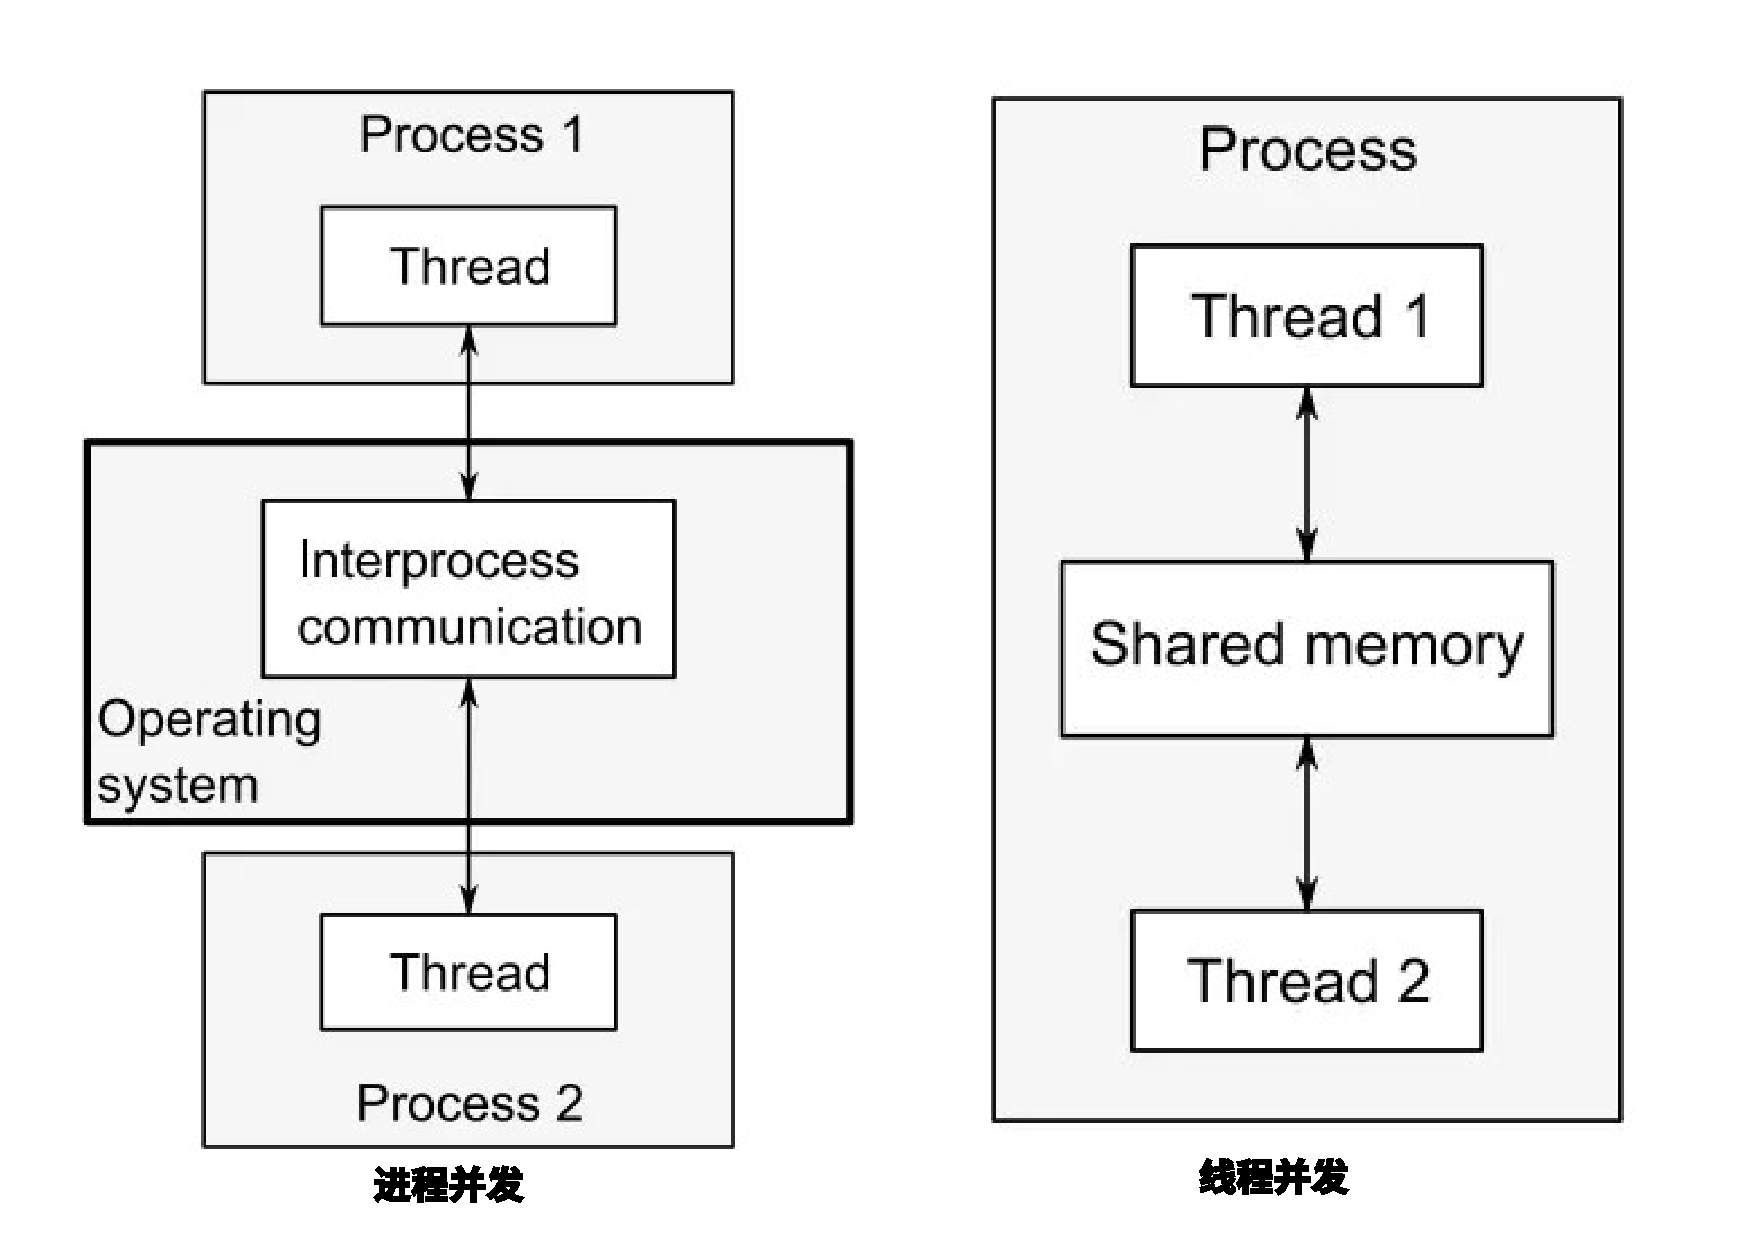
\includegraphics[scale=0.5]{Concurrency}
	\caption{进程并发与线程并发}
	\label{fig.concurrenncy}
\end{figure}
C++98标准中并没有线程库的存在,而在C++11中终于提供了多线程的标准库,提供了管理线程、保护共享数据、线程间同步操作、原子操作等类。多线程库对应的头文件是<\textbf{thread}>,类名为\textbf{std::thread}。现在假设我们有一个函数function1(),单线程串行运行该程序的代码为:\\
\begin{lstlisting}
#include <iostream>
#include <thread>

void function_1() {
	std::cout << "I'm function_1()" << std::endl;
}

int main() {
	function_1();
	return 0;
}
\end{lstlisting}
这里我们并没有使用thread的相关功能去开辟和管理线程,这是因为main()函数本身即为一个线程,成为主线程,所有的程序会在主线程中顺序运行。若我们向让function1()在其他线程中运行,可以按如下方式改写:\\
\begin{lstlisting}
#include <iostream>
#include <thread>

void function_1() {
	std::cout << "I'm function_1()" << std::endl;
}

int main() {
	std::thread t1(function_1);//开辟一个线程t1并运行函数function1
	// do other things
	std::cout << "main() before" << std::endl;
	std::cout << "main() before" << std::endl;
	std::cout << "main() before:" << std::endl;
	t1.join();//
	std::cout << "main() after" << std::endl;
	return 0;
}
\end{lstlisting}
代码分析:
\begin{enumerate}
	\item 首先使用std::thread name(fcn)函数创建一个\textbf{线程对象},fcn称为线程对象的\textbf{入口函数},该函数的运行周期即为线程的生命周期。
	\item 当线程对象t1创建后,对应的线程函数function1()即开始同步运行,函数运行结束即标志着\textbf{线程}结束,但\textbf{线程对象}并未释放;
	\item main线程和t1线程是同步执行的,但两个线程并不是同时结束的,因此需要在main函数中设定线程的执行类型。线程的类型包括join()和detach()两种;join()称为线程等待函数,main线程在同步运行至join()函数时,会判断对应的t1线程是否运行完成;若完成子继续运行main线程中join()后的内容,否则等待t1线程运行。与之相对,detach()称为线程分离函数,main线程运行至detach()时会将t1线程分离出去,随即继续运行main线程的后续内容。
\end{enumerate}
\subsection{线程构造函数}
线程构造函数std::thread()是一个可变参数函数,第一个参数为线程的入口函数,后面参数以此为入口函数的对应参数,例如:
\begin{lstlisting}
// 普通函数 无参
void function_1() {
}

// 普通函数 1个参数
void function_2(int i) {
}

// 普通函数 2个参数
void function_3(int i, std::string m) {
}

std::thread t1(function_1);
std::thread t2(function_2, 1);
std::thread t3(function_3, 1, "hello");

t1.join();
t2.join();
t3.join();
\end{lstlisting}
需要注意的是,线程的入口函数不接受重载函数,重载函数会使得编译器无法决定正确的函数类型从而引发编译错误。

此外,入口函数还可以是仿函数、匿名函数和std::function对象。
\begin{enumerate}
	\item 仿函数:
	\begin{lstlisting}
		// 仿函数
		class Fctor {
		public:
		// 具有一个参数
		void operator() () {
		
		}
		};
		Fctor f;
		std::thread t1(f);  
		// std::thread t2(Fctor()); // 编译错误 
		std::thread t3((Fctor())); // ok
		std::thread t4{Fctor()}; // ok
	\end{lstlisting}
	\item 匿名函数:
	\begin{lstlisting}
		std::thread t1([](){
		std::cout << "hello" << std::endl;
		});
		
		std::thread t2([](std::string m){
		std::cout << "hello " << m << std::endl;
		}, "world");
	\end{lstlisting}
	\item std::function:
	\begin{lstlisting}
		class A{
		public:
		void func1(){
		}
		
		void func2(int i){
		}
		void func3(int i, int j){
		}
		};
		
		A a;
		std::function<void(void)> f1 = std::bind(&A::func1, &a);
		std::function<void(void)> f2 = std::bind(&A::func2, &a, 1);
		std::function<void(int)> f3 = std::bind(&A::func2, &a, std::placeholders::_1);
		std::function<void(int)> f4 = std::bind(&A::func3, &a, 1, std::placeholders::_1);
		std::function<void(int, int)> f5 = std::bind(&A::func3, &a, std::placeholders::_1, std::placeholders::_2);
		
		std::thread t1(f1);
		std::thread t2(f2);
		std::thread t3(f3, 1);
		std::thread t4(f4, 1);
		std::thread t5(f5, 1, 2);
	\end{lstlisting}
\end{enumerate}

注1:需要注意的是,线程入口函数传入的参数只有\textbf{传值}一种类型,即便入口函数的参数是引用形式,为了保证线程数据的安全性,新开辟线程也会在构造线程兑现对传入的数值进行拷贝。
注2:线程对象之间是不能复制的,只能移动,移动的意思是,将线程的所有权在std::thread实例间进行转移。
\begin{lstlisting}
	void some_function();
	void some_other_function();
	std::thread t1(some_function);
	// std::thread t2 = t1; // 编译错误
	std::thread t2 = std::move(t1); //只能移动 t1内部已经没有线程了
	t1 = std::thread(some_other_function); // 临时对象赋值 默认就是移动操作
	std::thread t3;
	t3 = std::move(t2); // t2内部已经没有线程了
	t1 = std::move(t3); // 程序将会终止,因为t1内部已经有一个线程在管理了
\end{lstlisting}
\subsection{线程与竞争条件}
并发代码中最常见的错误之一就是竞争条件(race condition)。而其中最常见的就是数据竞争(data race),从整体上来看,所有线程之间共享数据的问题,都是修改数据导致的,如果所有的共享数据都是只读的,就不会发生问题。但是这是不可能的,大部分共享数据都是要被修改的。

std::cout()就是一个典型的共享资源对象,其操作基于数据流实现:\\
\begin{lstlisting}
#include <iostream>
#include <thread>
#include <string>
using namespace std;

// 普通函数 无参
void function_1() {
for(int i=0; i>-100; i--)
	cout << "From t1: " << i << endl;
}

int main()
{
	std::thread t1(function_1);
	
	for(int i=0; i<100; i++)
		cout << "From main: " << i << endl;
	
	t1.join();
	return 0;
}
\end{lstlisting}
在上面这里demo中,运行结果会出现如下的混乱情况,这是因为cout的数据流在两个线程中是共享的,两个线程执行cout取出数据的时机是完全随机的:\\
\begin{lstlisting}
From main: 0
From main: 1From t1: 
From main: 2
\end{lstlisting}
c++中提供了解决这一问题的方式——互斥锁(Mutex),其包含在头文件<\textbf{mutex}>中,在使用共享资源前使用std::mutex.lock()锁定线程,使用完毕后使用std::mutex.unlock()解锁线程,即可保护共享资源对象:\\
\begin{lstlisting}
#include <iostream>
#include <thread>
#include <string>
#include <mutex>
using namespace std;

std::mutex mu;
// 使用锁保护
void shared_print(string msg, int id) {
	mu.lock(); // 上锁
	cout << msg << id << endl;
	mu.unlock(); // 解锁
}

void function_1() {
	for(int i=0; i>-100; i--)
		shared_print(string("From t1: "), i);
}

int main()
{
	std::thread t1(function_1);
	
	for(int i=0; i<100; i++)
		shared_print(string("From main: "), i);
	
	t1.join();
	return 0;
}	
\end{lstlisting}
但由用户手动加锁与解锁存在一个隐藏问题,即当lock于unlock之间的代码出现异常退出时,系统不会自动将共享资源解锁,时候后续需要使用该共享资源的线程秩序堵塞。C++标准库提供了lock\_guard模板类解决这一问题,该模板类是c++中常见的RAII技术,即获取资源即初始化(Resource Acquisition Is Initialization)技术。该模板类在创建类对象的时候会自动对线程加锁,在对象析构时,则会自动对线程解锁。\\
\begin{lstlisting}
void shared_print(string msg, int id) {
	//构造的时候帮忙上锁
	std::lock_guard<std::mutex> guard(mu);
	
	cout << msg << id << endl;
	//即便代码出现异常退出,由于函数运行结束,函数内创建的lock_guard对象
	//释放时会自动调用析构函数,保证线程解锁
}
\end{lstlisting}
同时,由于mutex本身是一个全局变量,但其服务对象仅为shared\_print函数,因此可以将两者分别封装为类的成员变量和成员函数,以优化代码:\\
\begin{lstlisting}
#include <iostream>
#include <thread>
#include <string>
#include <mutex>
#include <fstream>
using namespace std;

std::mutex mu;
class LogFile {
std::mutex m_mutex;
ofstream f;
public:
LogFile() {
f.open("log.txt");
}
~LogFile() {
f.close();
}
void shared_print(string msg, int id) {
std::lock_guard<std::mutex> guard(mu);
f << msg << id << endl;
}
};

void function_1(LogFile& log) {
for(int i=0; i>-100; i--)
log.shared_print(string("From t1: "), i);
}

int main()
{
LogFile log;
//log对象不能拷贝,需要使用ref传入原引用
std::thread t1(function_1, std::ref(log));

for(int i=0; i<100; i++)
log.shared_print(string("From main: "), i);

t1.join();
return 0;
}
\end{lstlisting}
上一节我们提到过,线程函数的参数本质是拷贝而非赋值。这里由于ofstream对象不能直接拷贝,需要使用std::ref()函数将原对象的引用传入。
\subsection{死锁}
将mutex上锁而不解锁的情况称为\textbf{死锁},这种情况下使用lock\_guard可以保证析构的时候能够释放锁,然而,当一个操作需要使用两个互斥锁的时候,仅仅使用lock\_guard并不能保证不会发生死锁,如下面的例子:
\begin{lstlisting}
#include <iostream>
#include <thread>
#include <string>
#include <mutex>
#include <fstream>
using namespace std;

class LogFile {
	std::mutex _mu;
	std::mutex _mu2;
	ofstream f;
public:
	LogFile() {
		f.open("log.txt");
	}
	~LogFile() {
		f.close();
	}
	void shared_print(string msg, int id) {
		std::lock_guard<std::mutex> guard(_mu);
		std::lock_guard<std::mutex> guard2(_mu2);
		f << msg << id << endl;
		cout << msg << id << endl;
	}
	void shared_print2(string msg, int id) {
		std::lock_guard<std::mutex> guard(_mu2);
		std::lock_guard<std::mutex> guard2(_mu);
		f << msg << id << endl;
		cout << msg << id << endl;
	}
};

void function_1(LogFile& log) {
	for(int i=0; i>-100; i--)
		log.shared_print2(string("From t1: "), i);
}

int main()
{
	LogFile log;
	std::thread t1(function_1, std::ref(log));
	
	for(int i=0; i<100; i++)
		log.shared_print(string("From main: "), i);
	
	t1.join();
	return 0;
}
\end{lstlisting}
该demo中由于同时使用了两个互斥锁,在某些状况下会出现嵌套死锁,应尽量避免。
\subsection{unique\_lock}
使用互斥锁虽然保证了共享数据的唯一性,但亦将并行操作变为了串行操作,降低了代码效率,因此需要谨慎的设计上锁的代码块。如果一段代码中有多个代码块需要频繁的加锁与解锁,由于lock\_guard只会在创建时上锁,在析构时解锁,就需要创建多个局部lock\_guard对象,例如:\\
\begin{lstlisting}
std::mutex _mu;
{
	std::lock_guard<std::mutex> guard(_mu);
	\\code....
}
{
	std::lock_guard<std::mutex> guard(_mu);
	\\code....	
}
{
	std::lock_guard<std::mutex> guard(_mu);
	\\code....
}
\end{lstlisting}
这无疑增加了代码的复杂度,降低了可阅读性。而使用unique\_lock则可有效改善这一问题。unique\_lock提供了lock()和unlock()接口,能记录现在处于上锁还是没上锁状态,在析构的时候,会根据当前状态来决定是否要进行解锁(lock\_guard就一定会解锁)。上面的代码修改如下:\\
\begin{lstlisting}
class LogFile {
	std::mutex _mu;
	ofstream f;
	public:
		LogFile() {
			f.open("log.txt");
		}
		~LogFile() {
			f.close();
		}
		void shared_print(string msg, int id) {
		
			std::unique_lock<std::mutex> guard(_mu);
			//do something 1
			guard.unlock(); //临时解锁
			//do something 2
			guard.lock(); //继续上锁
			// do something 3
			f << msg << id << endl;
			cout << msg << id << endl;
			// 结束时析构guard会临时解锁
			// 这句话可要可不要,不写,析构的时候也会自动执行
			// guard.ulock();
	}
};
\end{lstlisting}
可以看到,unique\_lock记录了当前锁的状态,在无需加锁的代码区域,可以使用unlock借口临时解锁,随后再重新加锁。但由于需要一直维护锁的状态,unique\_lock的执行效率比lock\_guard要低,因此能使用lock\_guard解决的代码应尽量使用lock\_guard。

同时需要注意的是,lock\_guard和unique\_lock均不能复制,但unique\_lock可以移动。
\subsection{条件变量}
在C++11以后的标准中,条件变量是实现线程同步管理的另一个有效方式,其通常和unique\_lock一同配套使用以避免线程间的竞争。使用条件变量需要包含头文件\textbf{condition\_variable},其主要包括两个重要的成员函数机制,等待和唤醒:\\
\begin{enumerate}
	\item 等待 
		\iitem wait():阻塞当前线程直到条件变量唤醒
		\iitem wait\_for():阻塞当前线程直到条件变量唤醒或到达一定时间
		\iitem wait\_until():阻塞当前线程直到条件变量唤醒或到达指定时间点
	\item 唤醒
		\iitem notify\_one():随机唤醒一个等待线程
		\iitem notify\_all():唤醒所有等待线程
\end{enumerate}
其中,所有wait函数接受参数均为std::unique\_lock<std::mutex>对象,且可以选择使用微词pred避免虚假唤醒,即:\\
\begin{lstlisting}
void wait( std::unique_lock<std::mutex>& lock );
//Predicate 谓词函数,可以普通函数或者lambda表达式
template< class Predicate >
void wait( std::unique_lock<std::mutex>& lock, Predicate pred );
\end{lstlisting}
% Bibliography.
% -------------
\newpage
\bibliographystyle{ieeetrsrt}

% Important: substitute your BiBTeX (*.bib) files below.
% ------------------------------------------------------
\bibliography{strings,konrad,manuals}

\end{document}
